\subsection{Run on GTEx}
\draft{Firstly the algorithm is run on a subset of $5$ tissues of GTEx}
\begin{figure}[htb!]
    \centering
    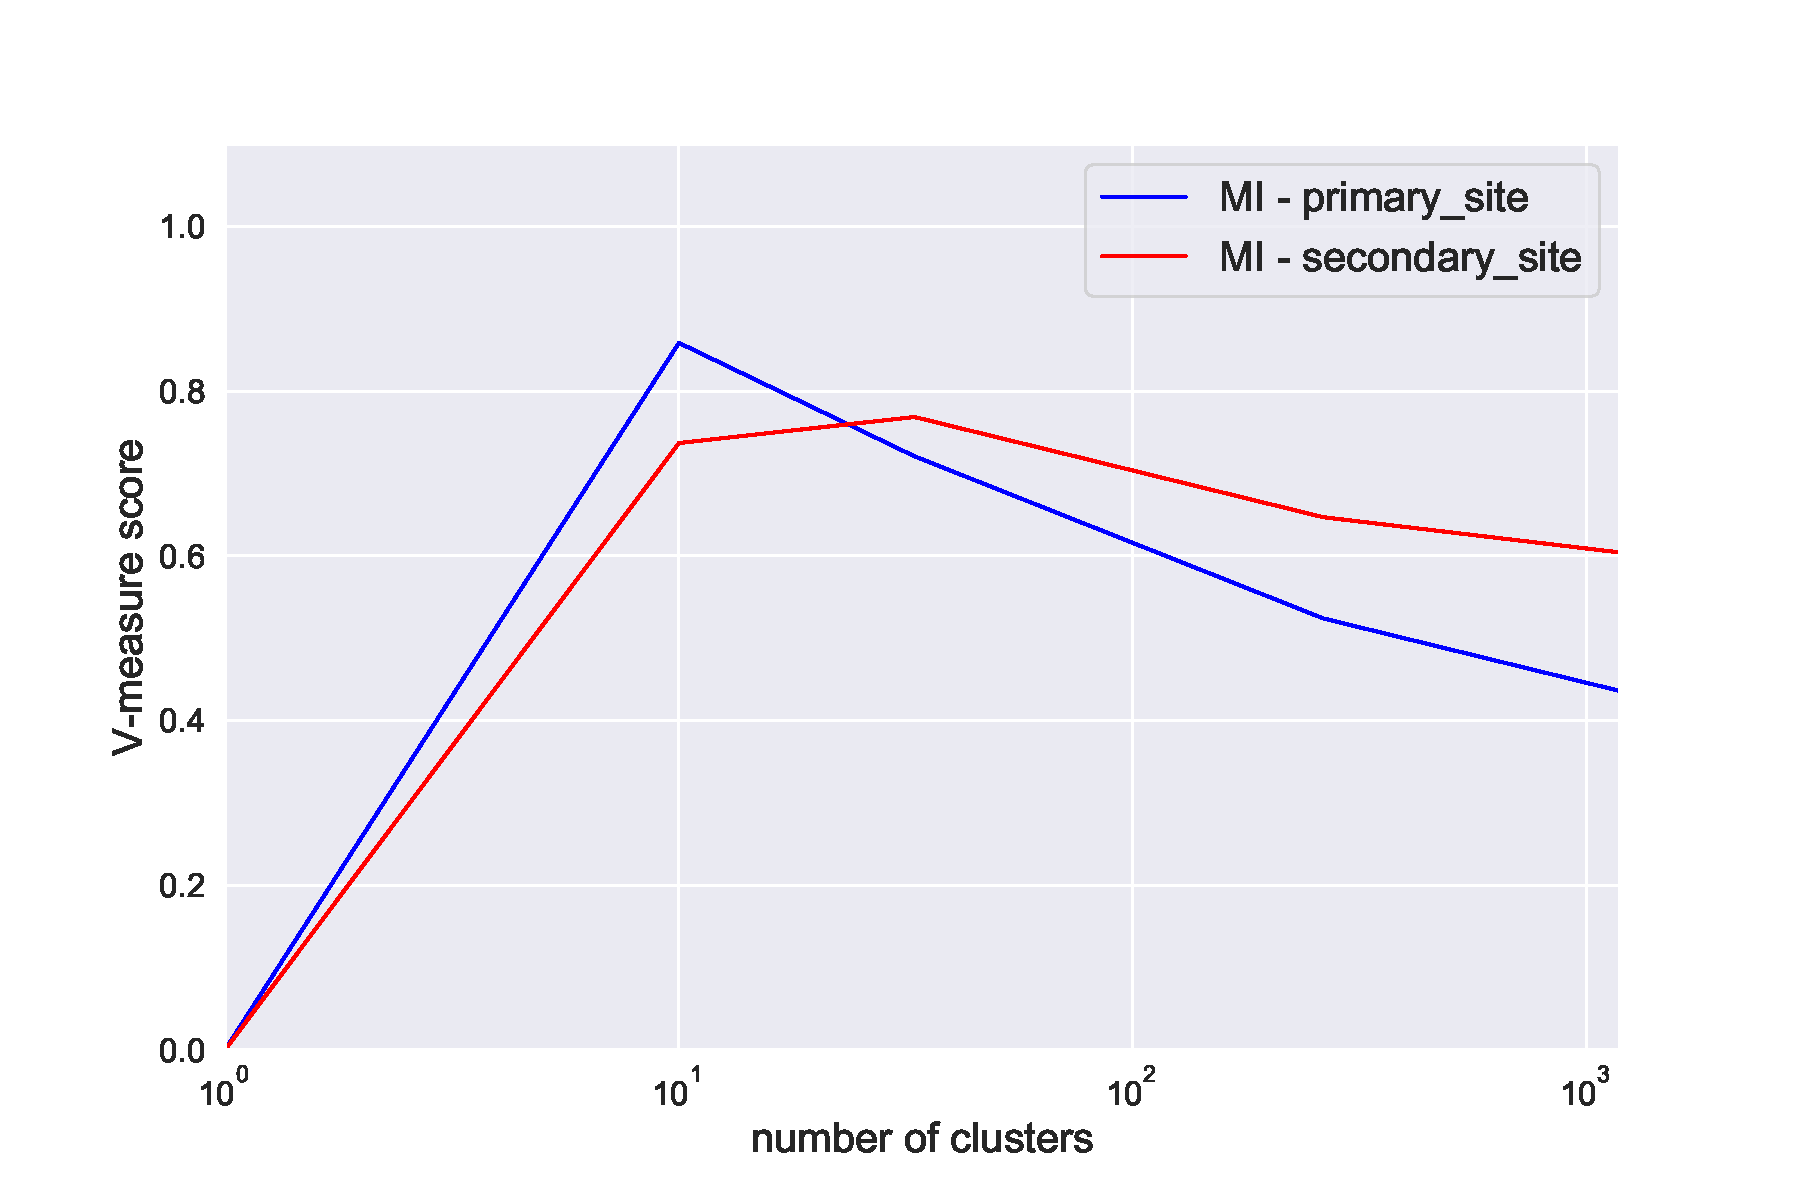
\includegraphics[width=0.9\linewidth]{pictures/topic/gtex/oversigma_10tissue/metric_scores.pdf}
    \caption{Scores across hierarchy}
    \label{fig:topic/gtex/oversigma_10tissue/metric_scores}
\end{figure}

\begin{figure}[htb!]
    \centering
    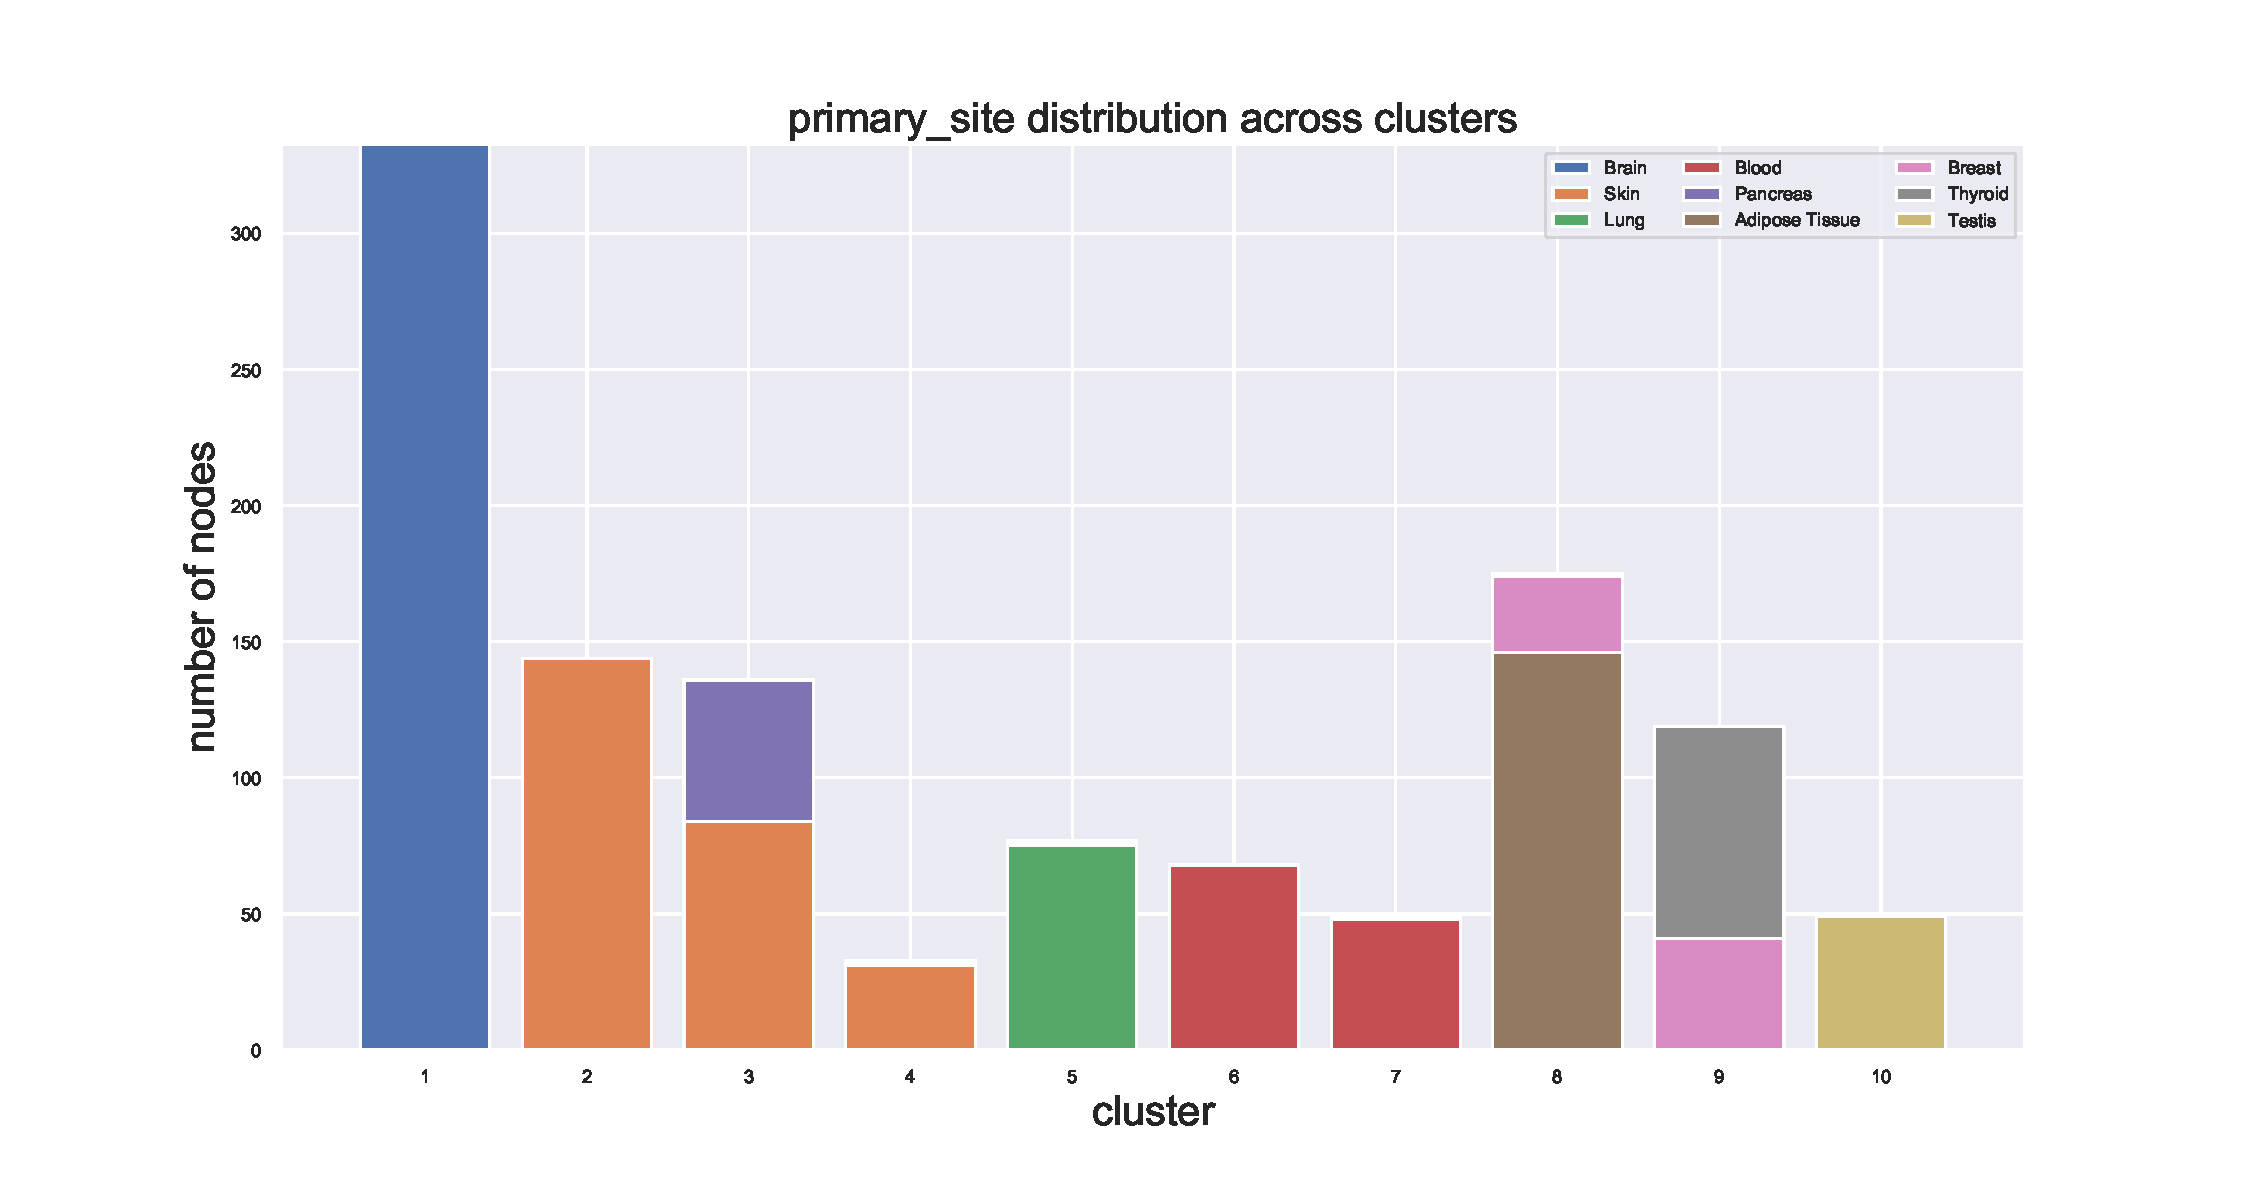
\includegraphics[width=0.9\linewidth]{pictures/topic/gtex/oversigma_10tissue/clustercomposition_l3_primary_site.pdf}
    \caption{Caption}
    \label{fig:topic/gtex/oversigma_10tissue/clustercomposition_l2_primary_site}
\end{figure}

\begin{figure}[htb!]
    \centering
    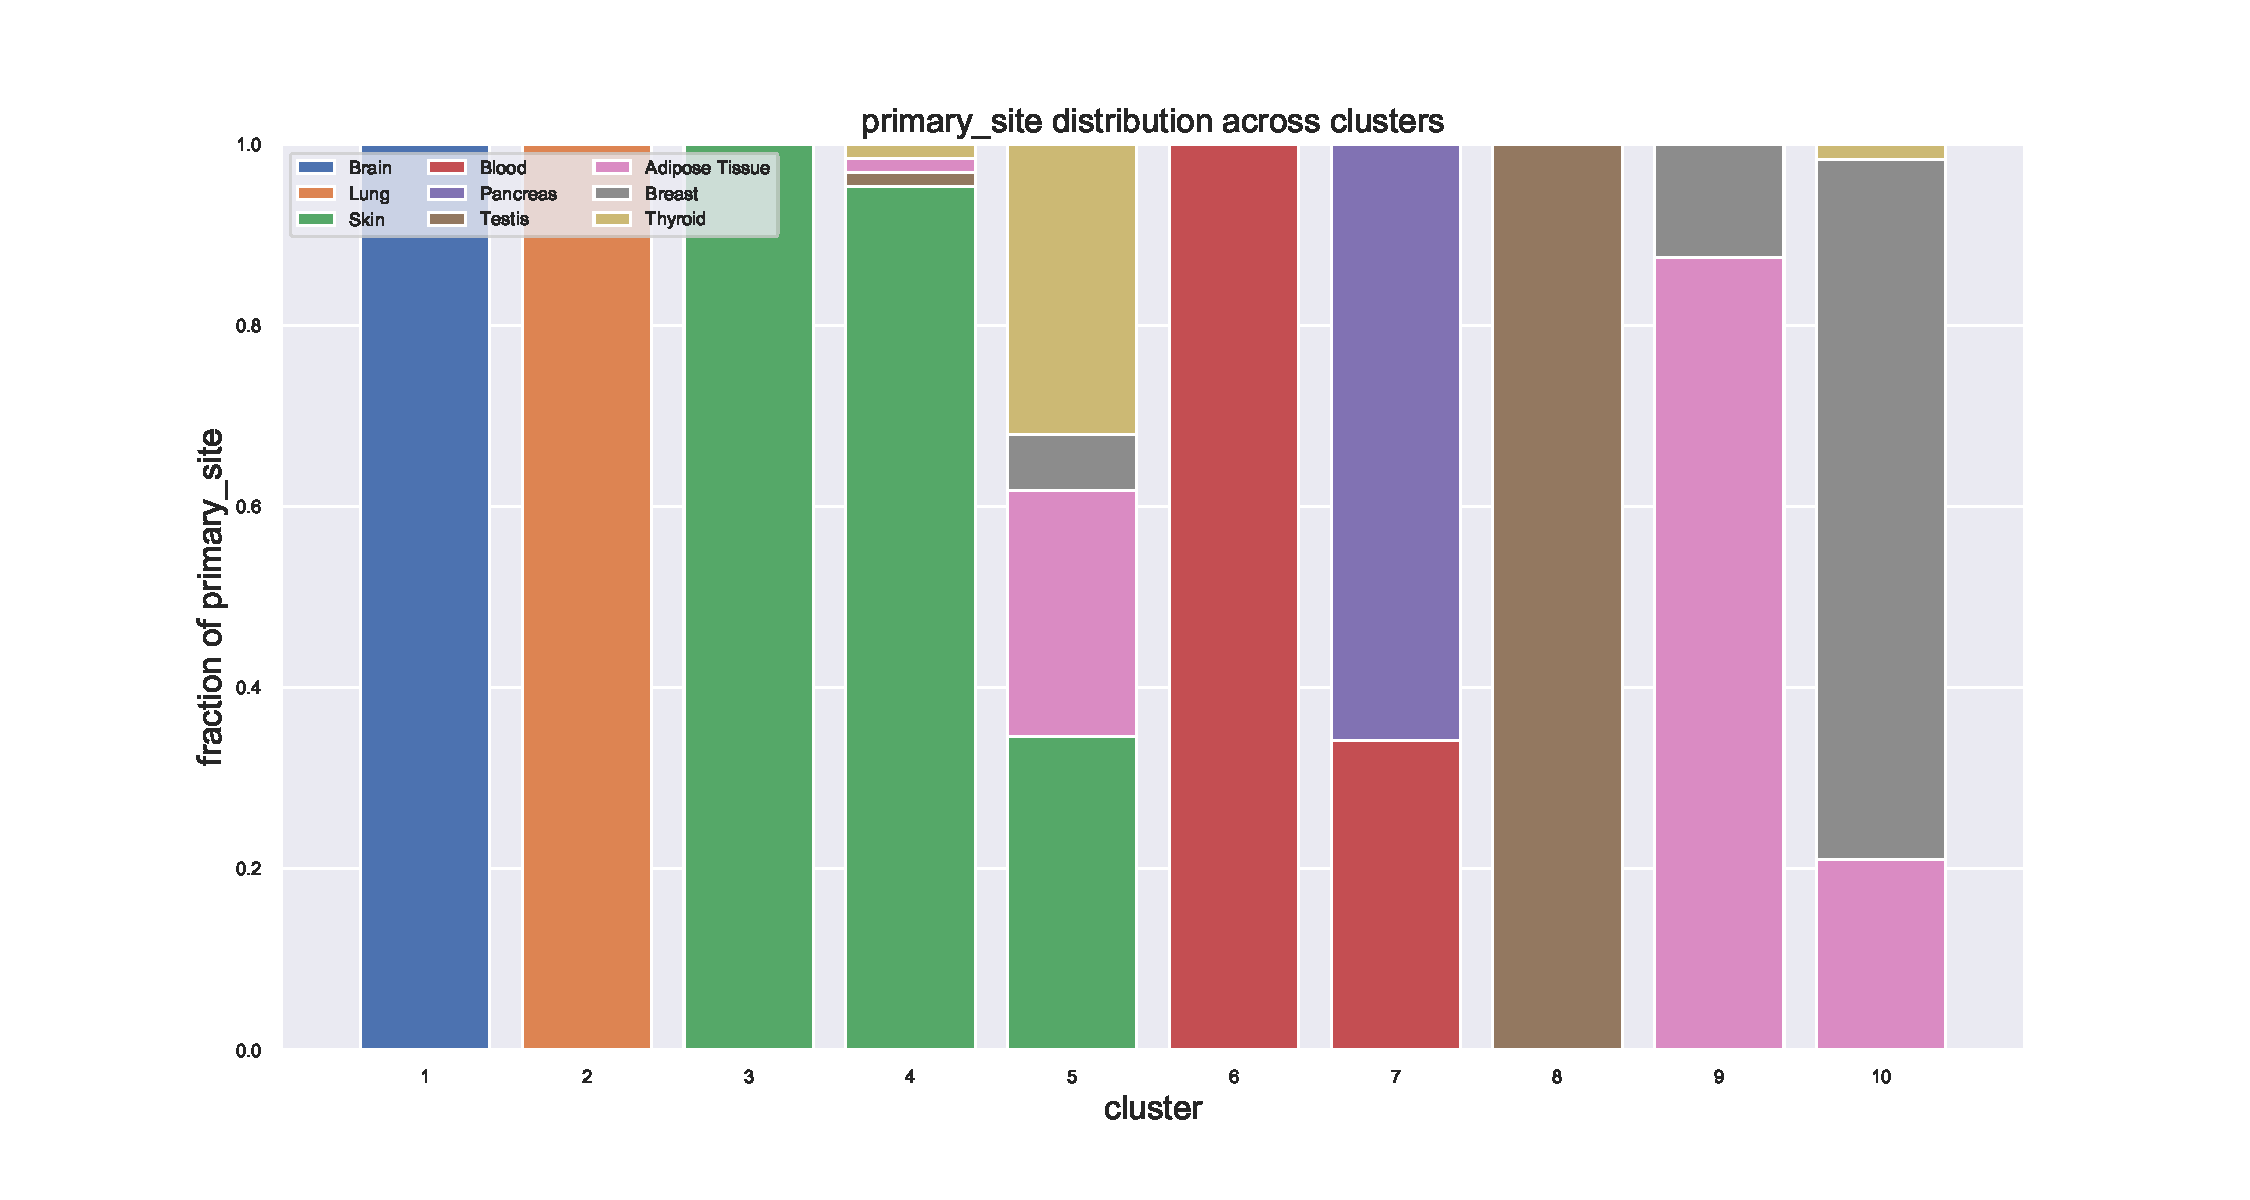
\includegraphics[width=0.9\linewidth]{pictures/topic/gtex/oversigma_10tissue/fraction_clustercomposition_l3_primary_site.pdf}
    \caption{Caption}
    \label{fig:topic/gtex/oversigma_10tissue/fraction_clustercomposition_l2_primary_site}
\end{figure}

\begin{figure}[htb!]
    \centering
    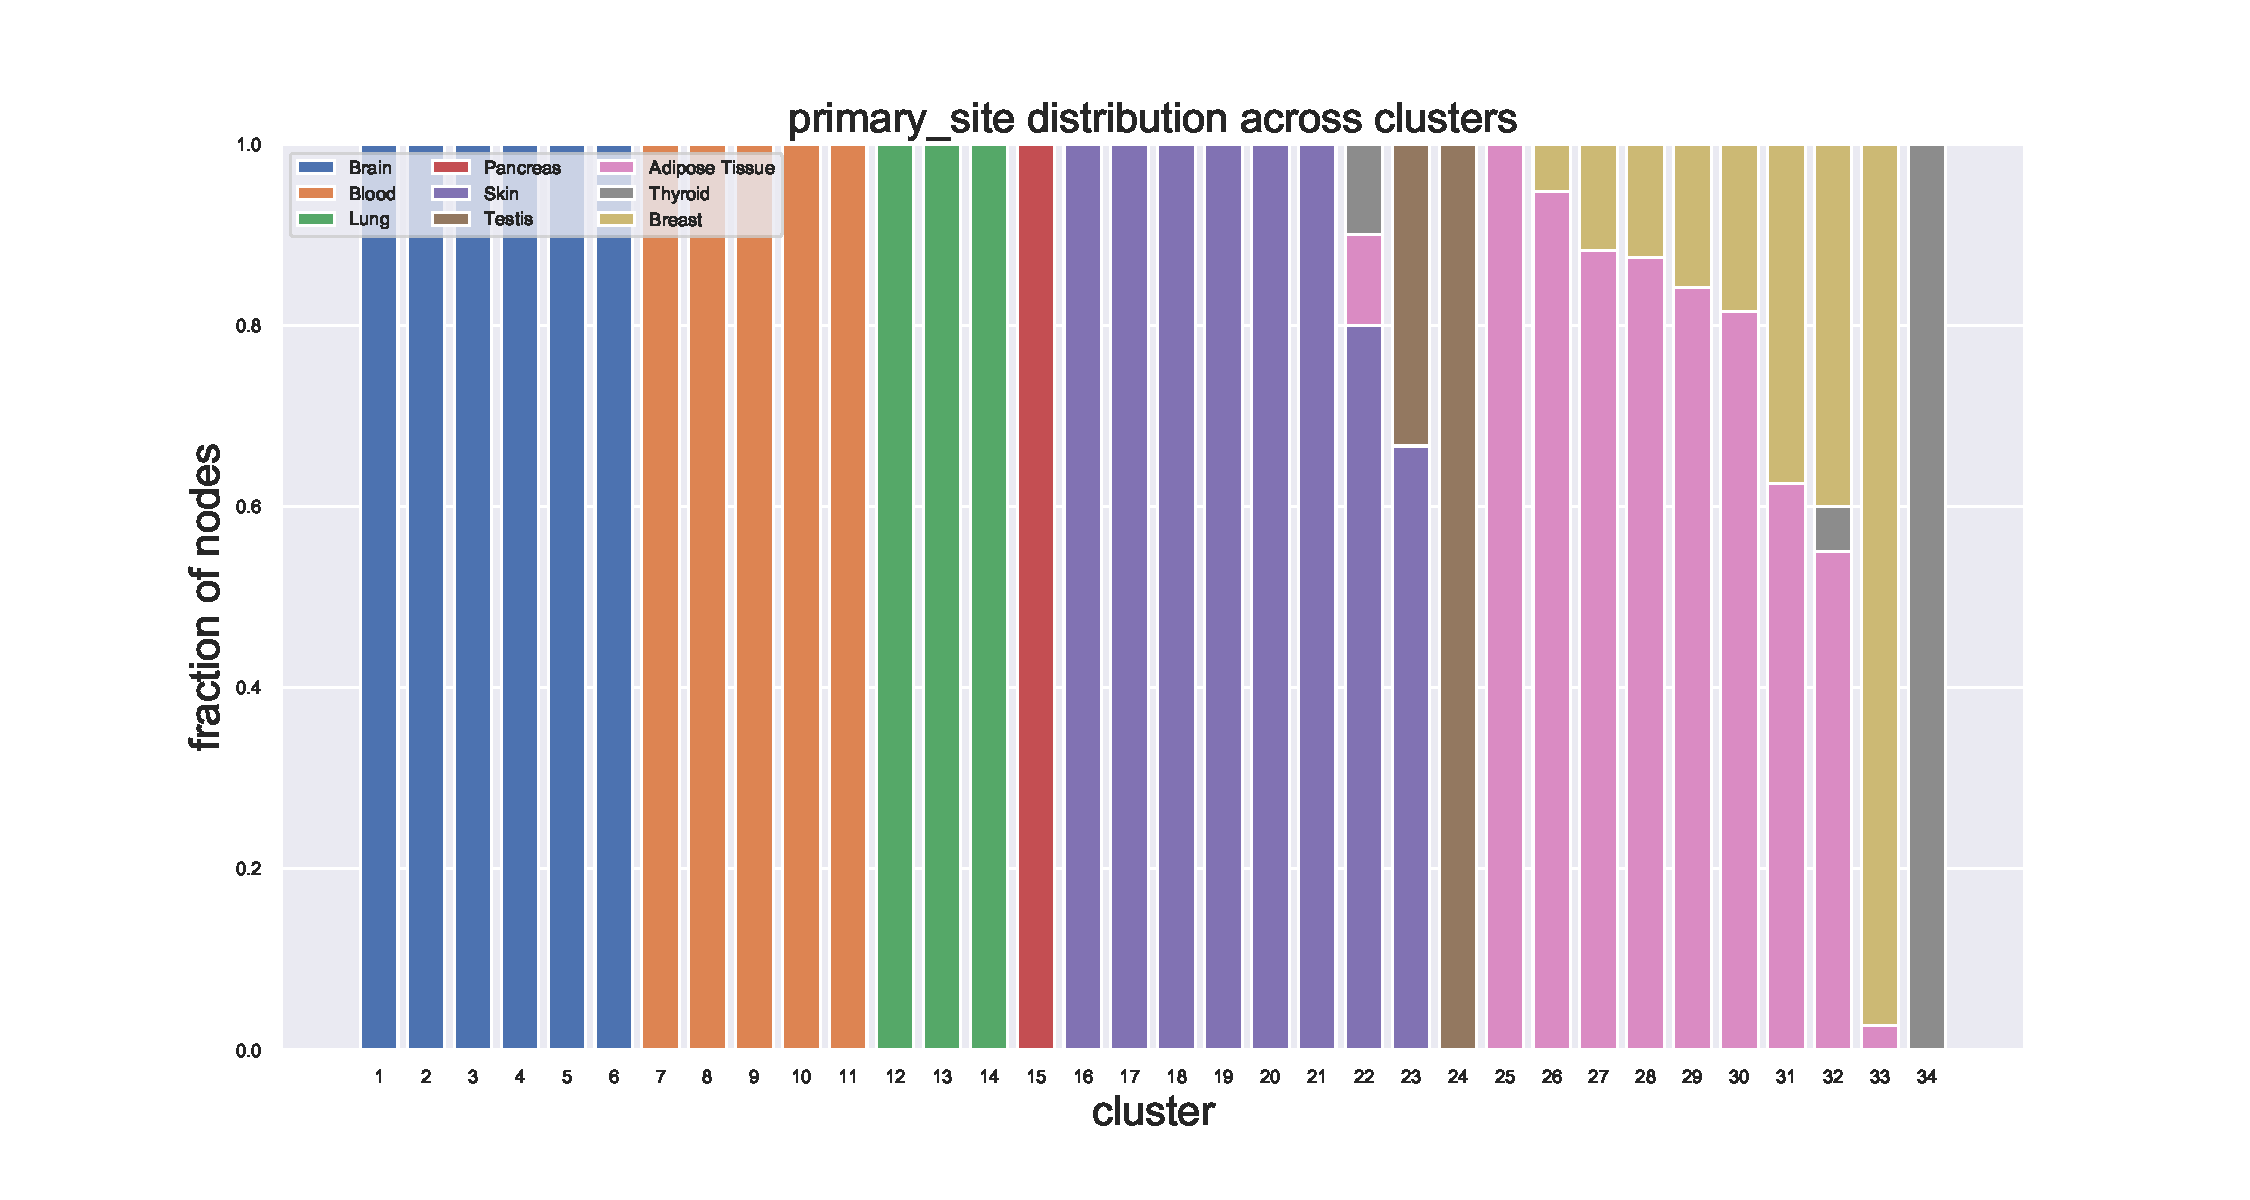
\includegraphics[width=0.9\linewidth]{pictures/topic/gtex/oversigma_10tissue/fraction_clustercomposition_l2_primary_site.pdf}
    \caption{Caption}
    \label{fig:topic/gtex/oversigma_10tissue/fraction_clustercomposition_l2_primary_site}
\end{figure}

\begin{figure}[htb!]
    \centering
    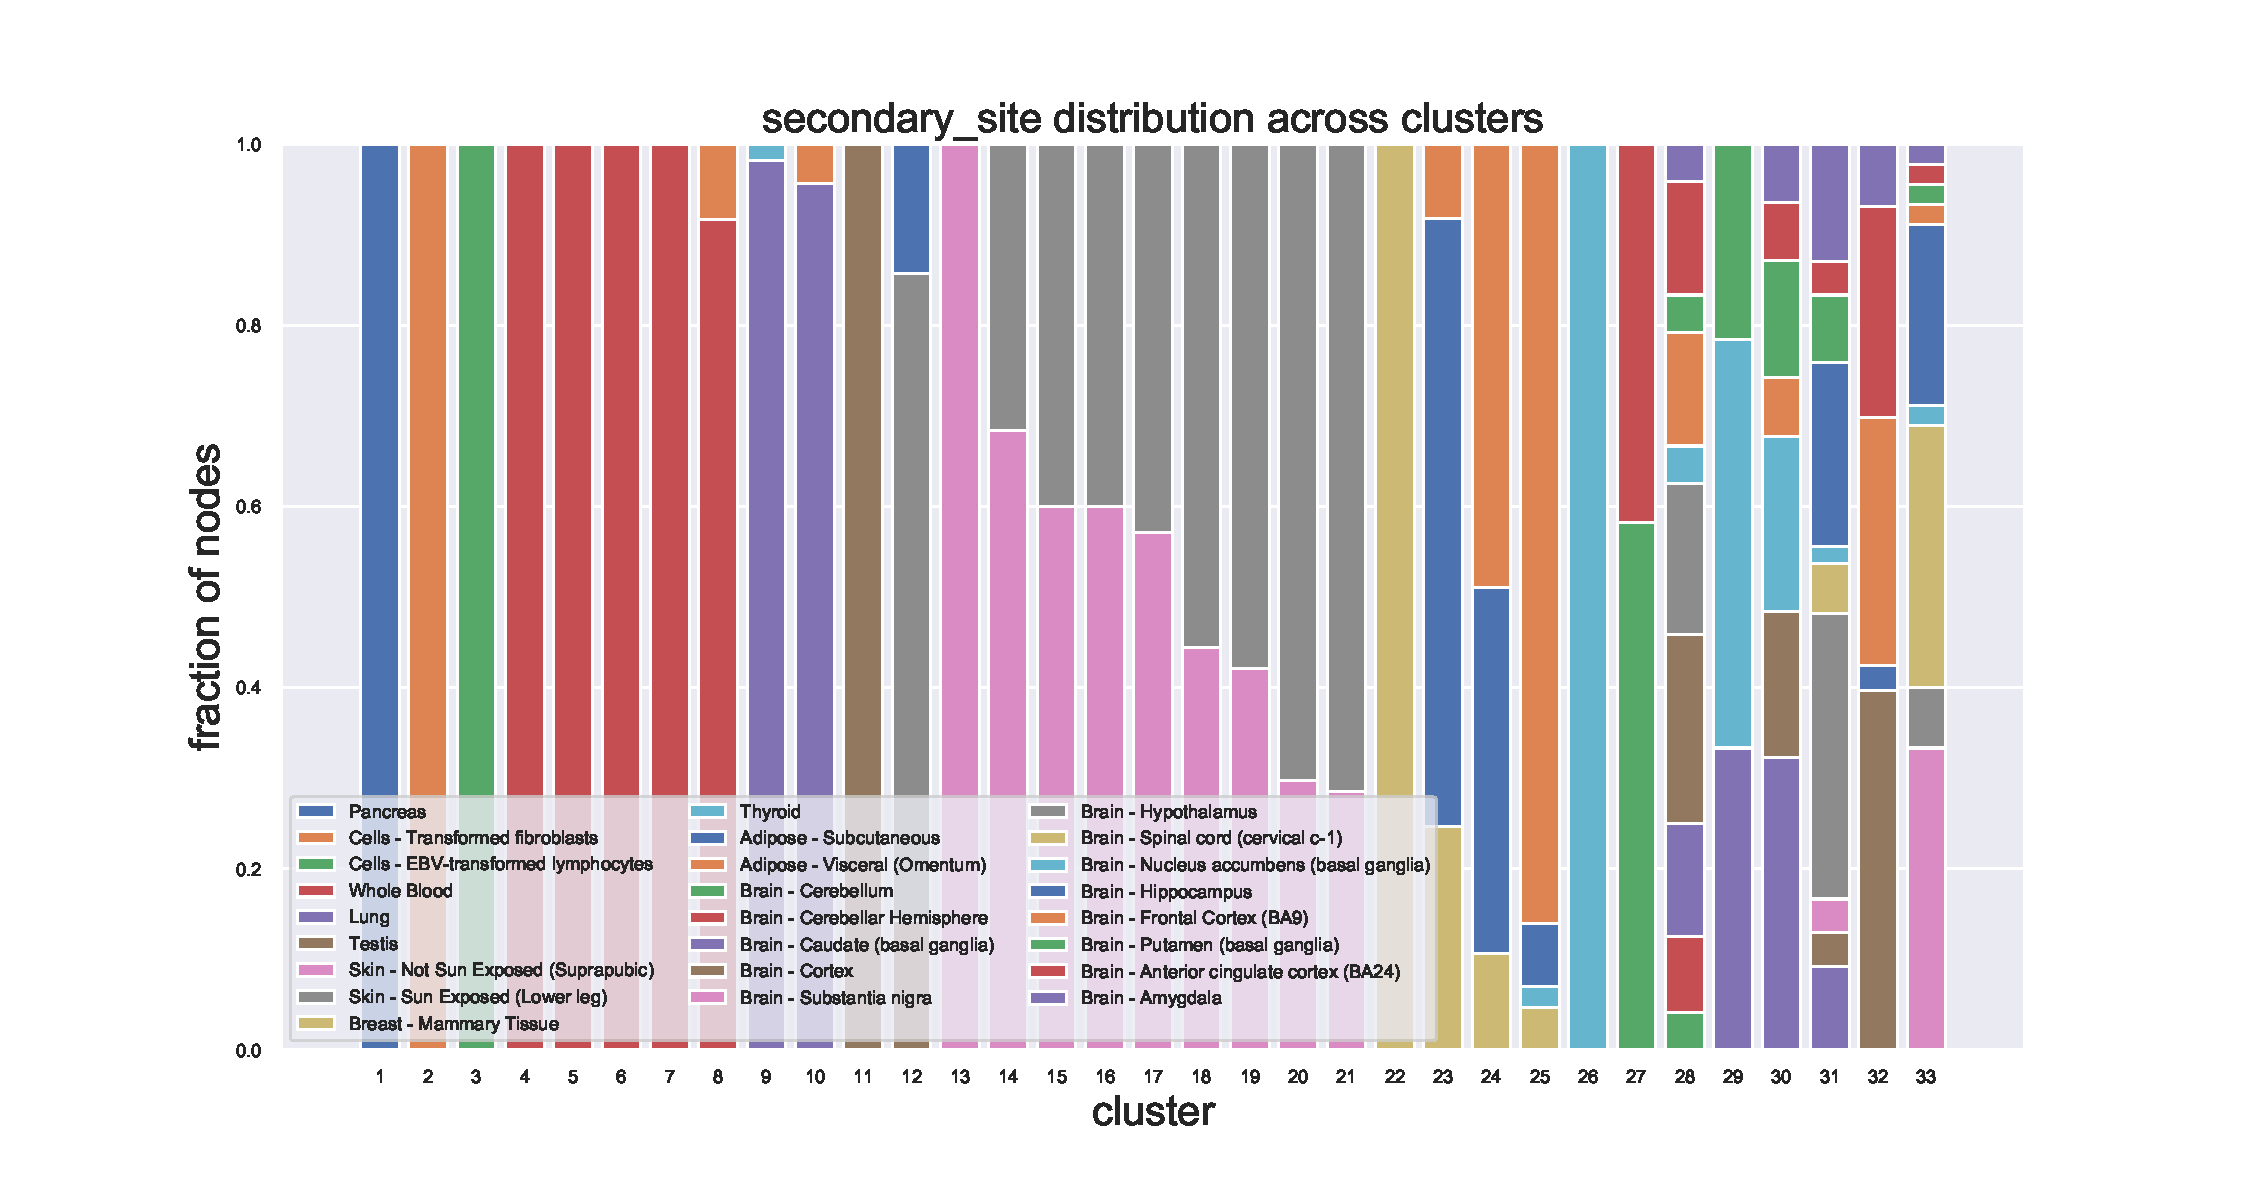
\includegraphics[width=0.9\linewidth]{pictures/topic/gtex/oversigma_10tissue/fraction_clustercomposition_l2_secondary_site.pdf}
    \caption{Caption}
    \label{fig:topic/gtex/oversigma_10tissue/fraction_clustercomposition_l2_secondary_site}
\end{figure}


\begin{figure}[htb!]
    \centering
    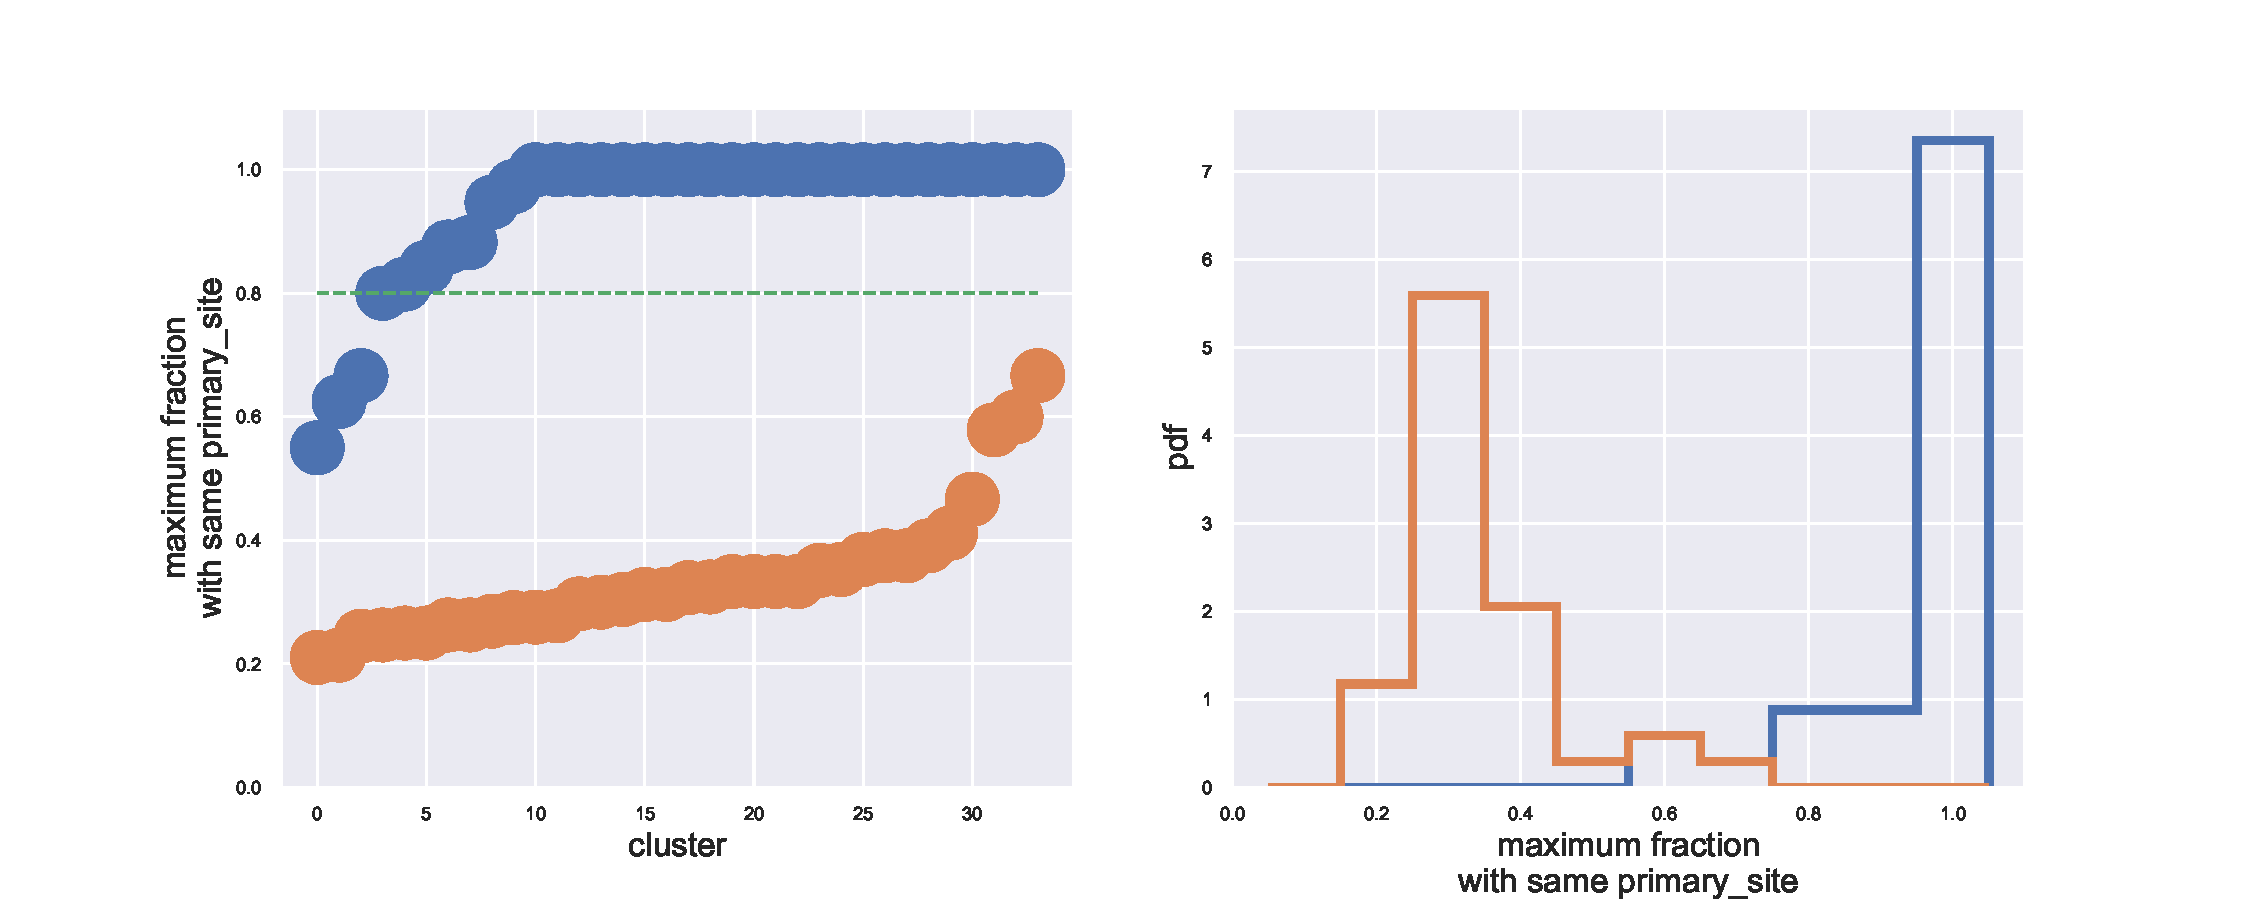
\includegraphics[width=0.9\linewidth]{pictures/topic/gtex/oversigma_10tissue/shuffledcluster_maximum_l2_primary_site.pdf}
    \caption{Caption}
    \label{fig:gtex/oversigma_10tissue/shuffledcluster_maximum_l2_primary_site}
\end{figure}

\begin{figure}[htb!]
    \centering
    \begin{minipage}{0.45\textwidth}
    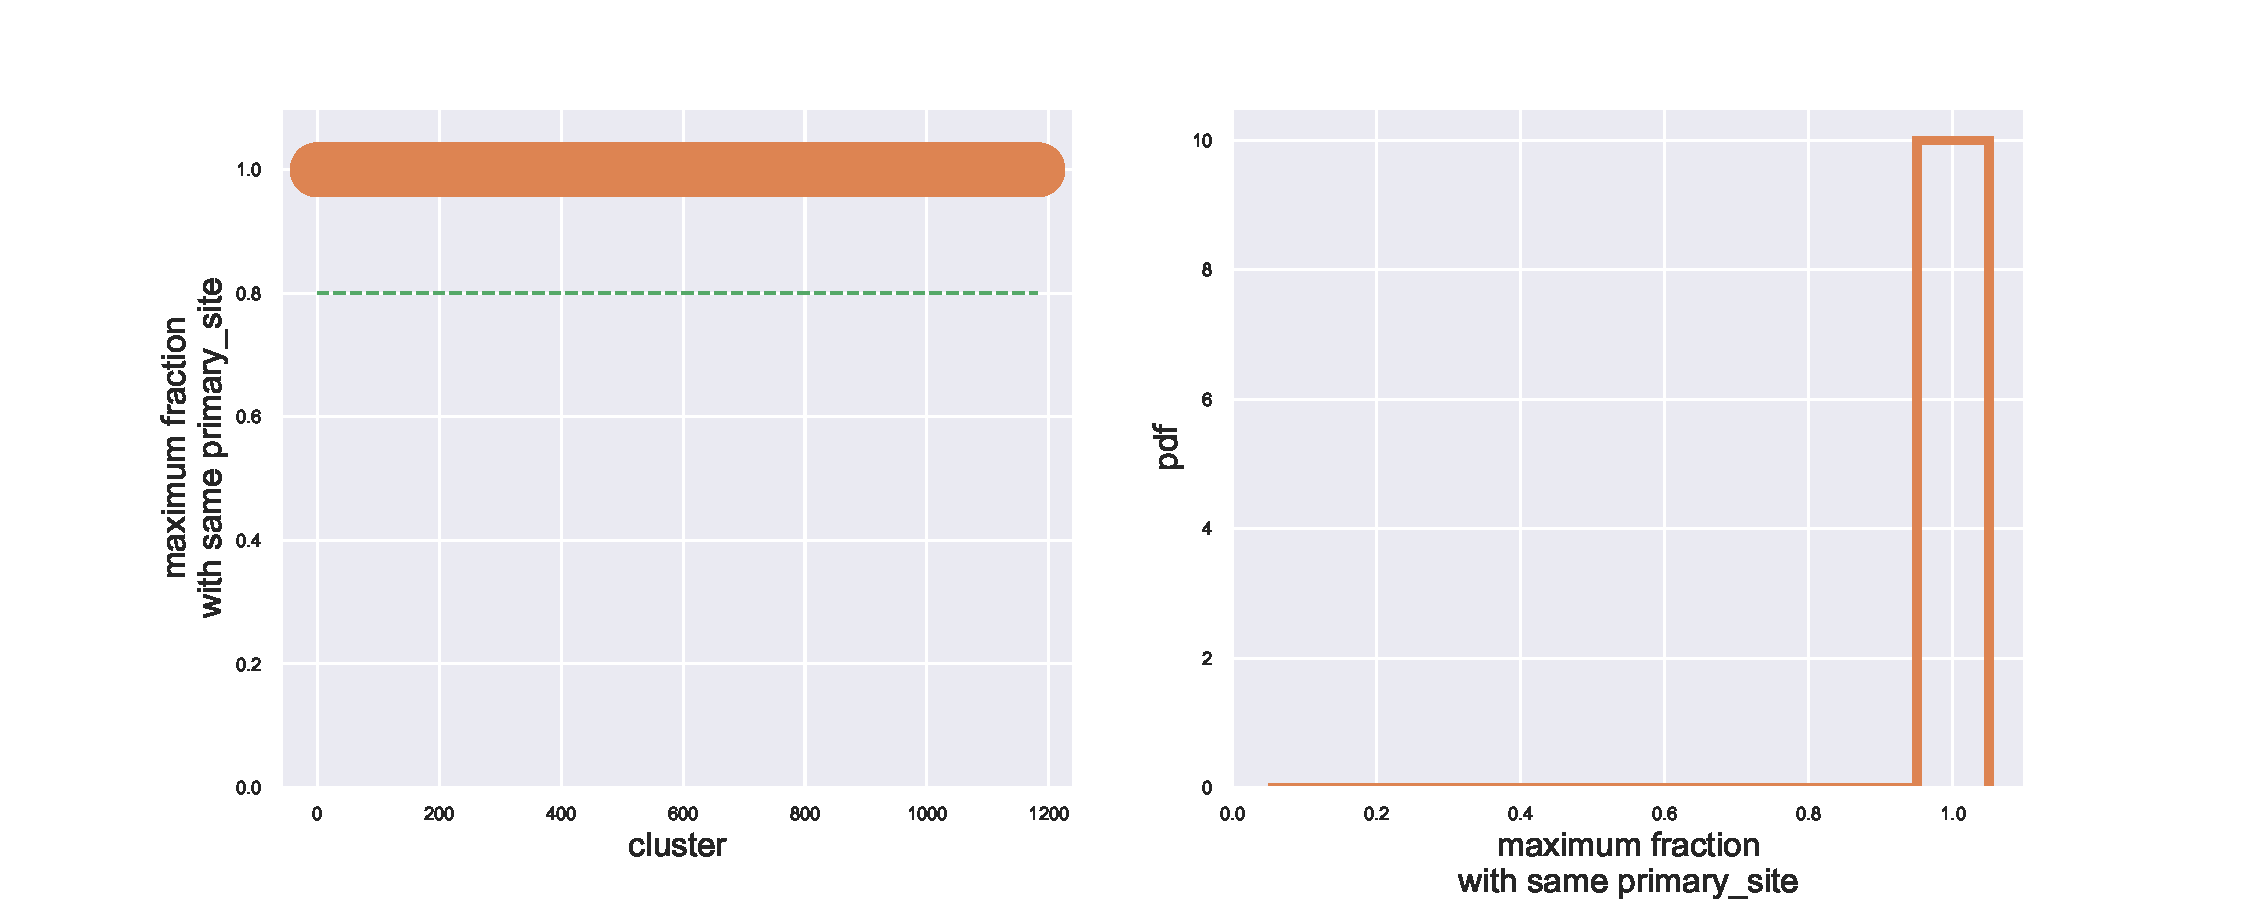
\includegraphics[width=0.9\linewidth]{pictures/topic/gtex/oversigma_10tissue/shuffledcluster_maximum_l0_primary_site.pdf}
    \end{minipage}
    \hspace{3mm}
    \begin{minipage}{0.45\textwidth}
    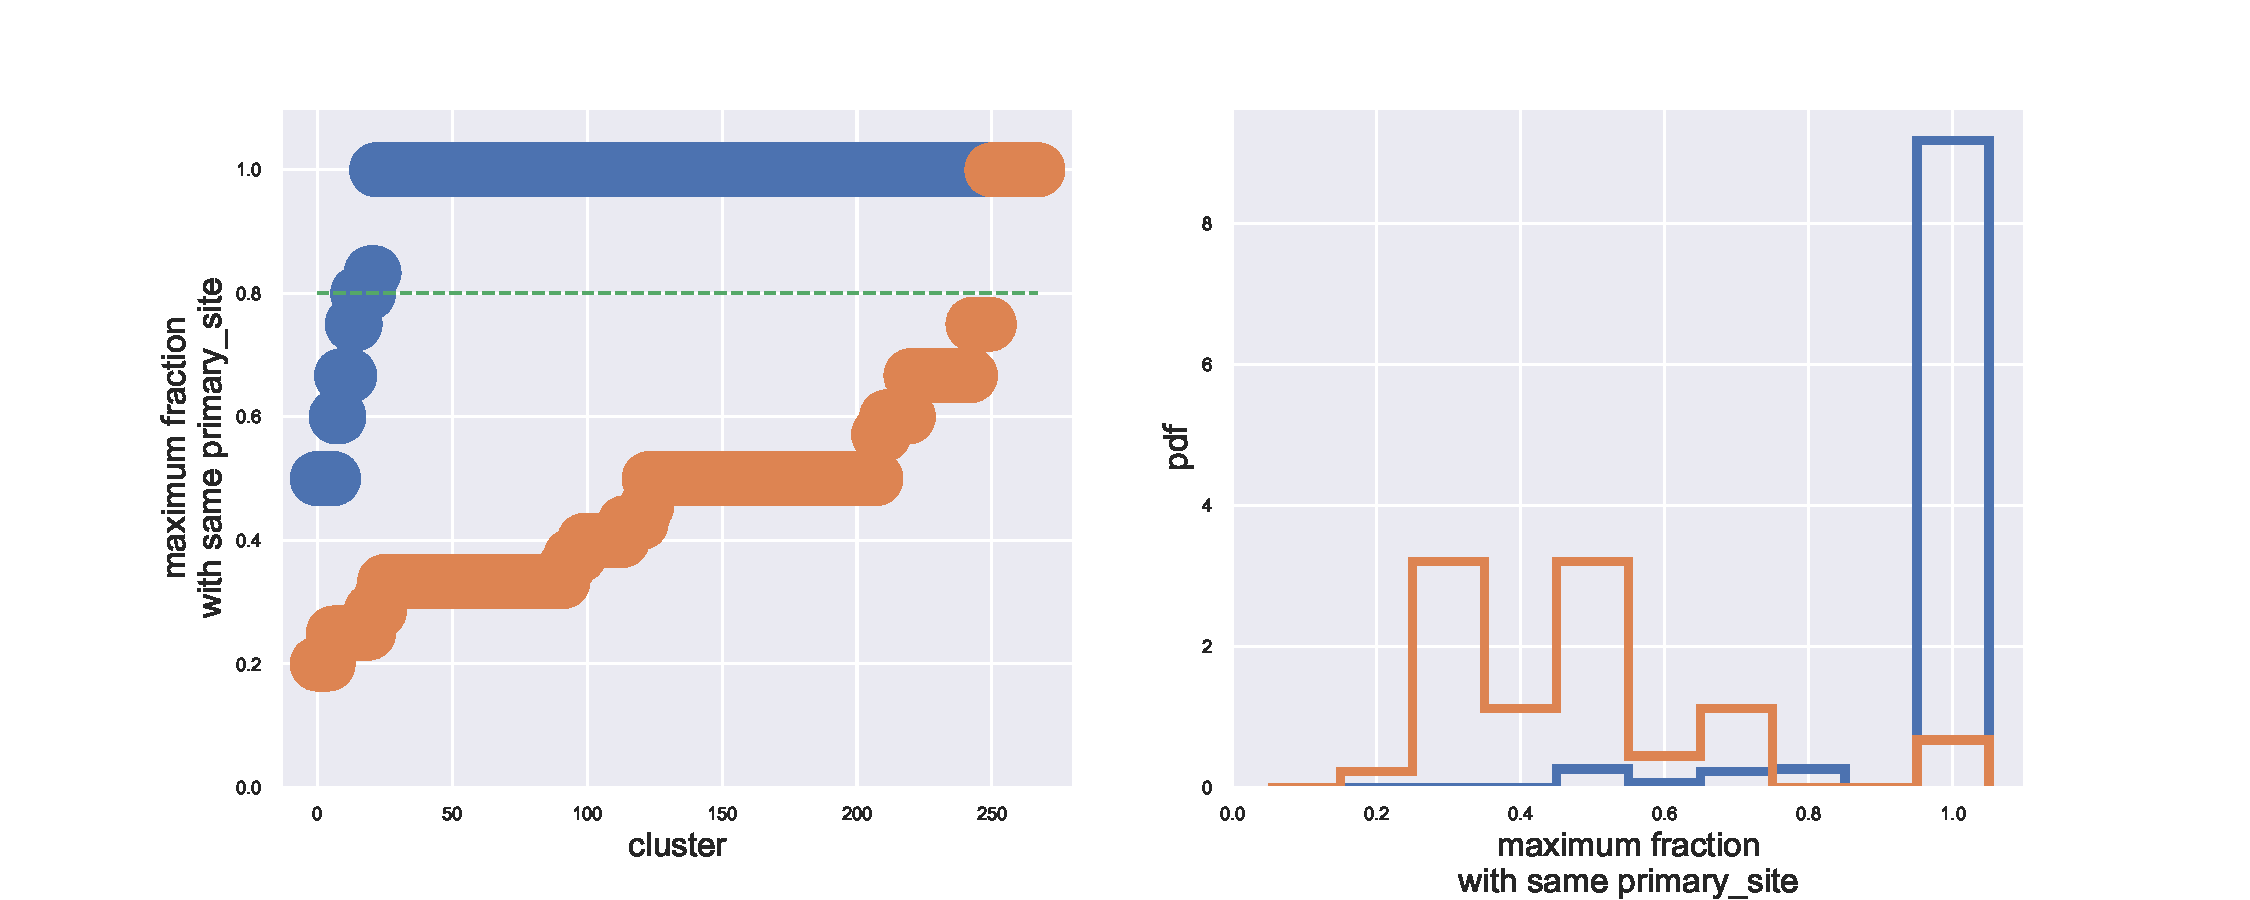
\includegraphics[width=0.9\linewidth]{pictures/topic/gtex/oversigma_10tissue/shuffledcluster_maximum_l1_primary_site.pdf}
    \end{minipage}
    \\
    \begin{minipage}{0.45\textwidth}
    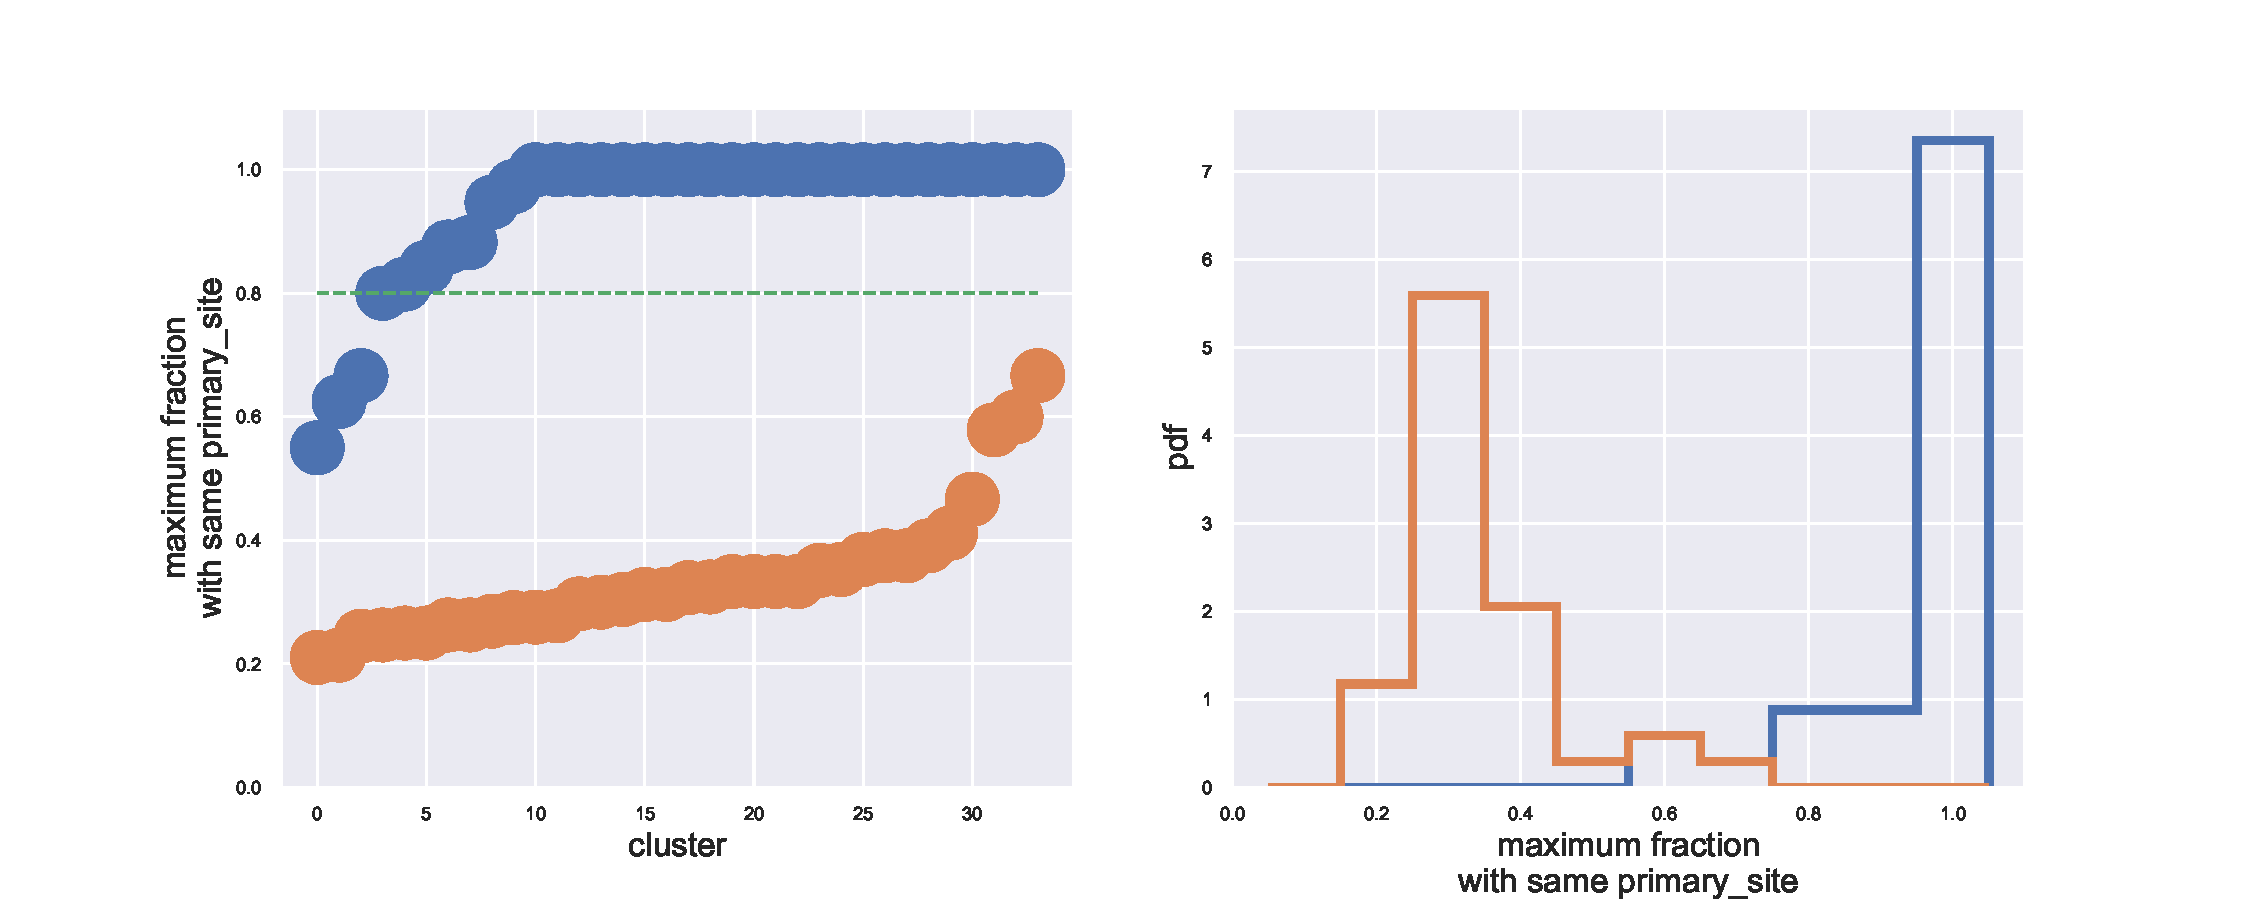
\includegraphics[width=0.9\linewidth]{pictures/topic/gtex/oversigma_10tissue/shuffledcluster_maximum_l2_primary_site.pdf}
    \end{minipage}
    \hspace{3mm}
    \begin{minipage}{0.45\textwidth}
    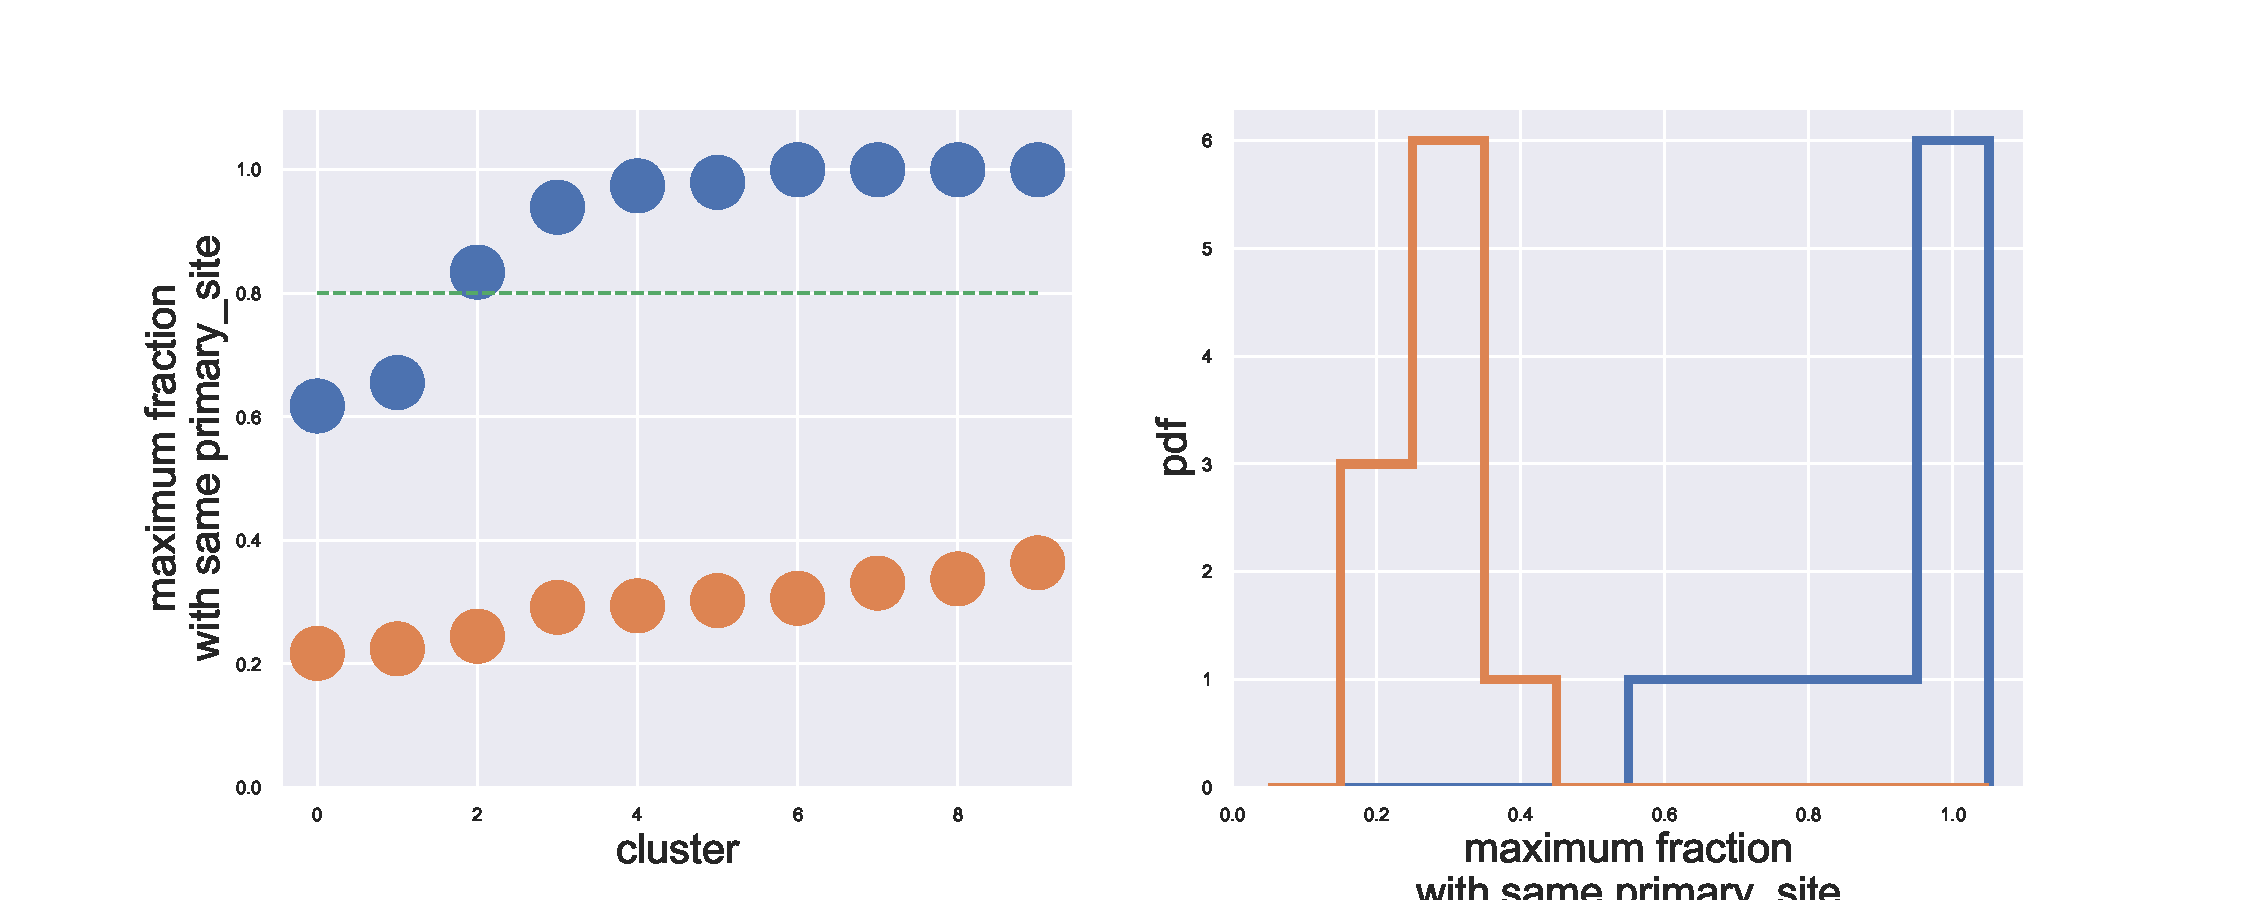
\includegraphics[width=0.9\linewidth]{pictures/topic/gtex/oversigma_10tissue/shuffledcluster_maximum_l3_primary_site.pdf}
    \end{minipage}
\end{figure}

\begin{figure}[htb!]
    \centering
    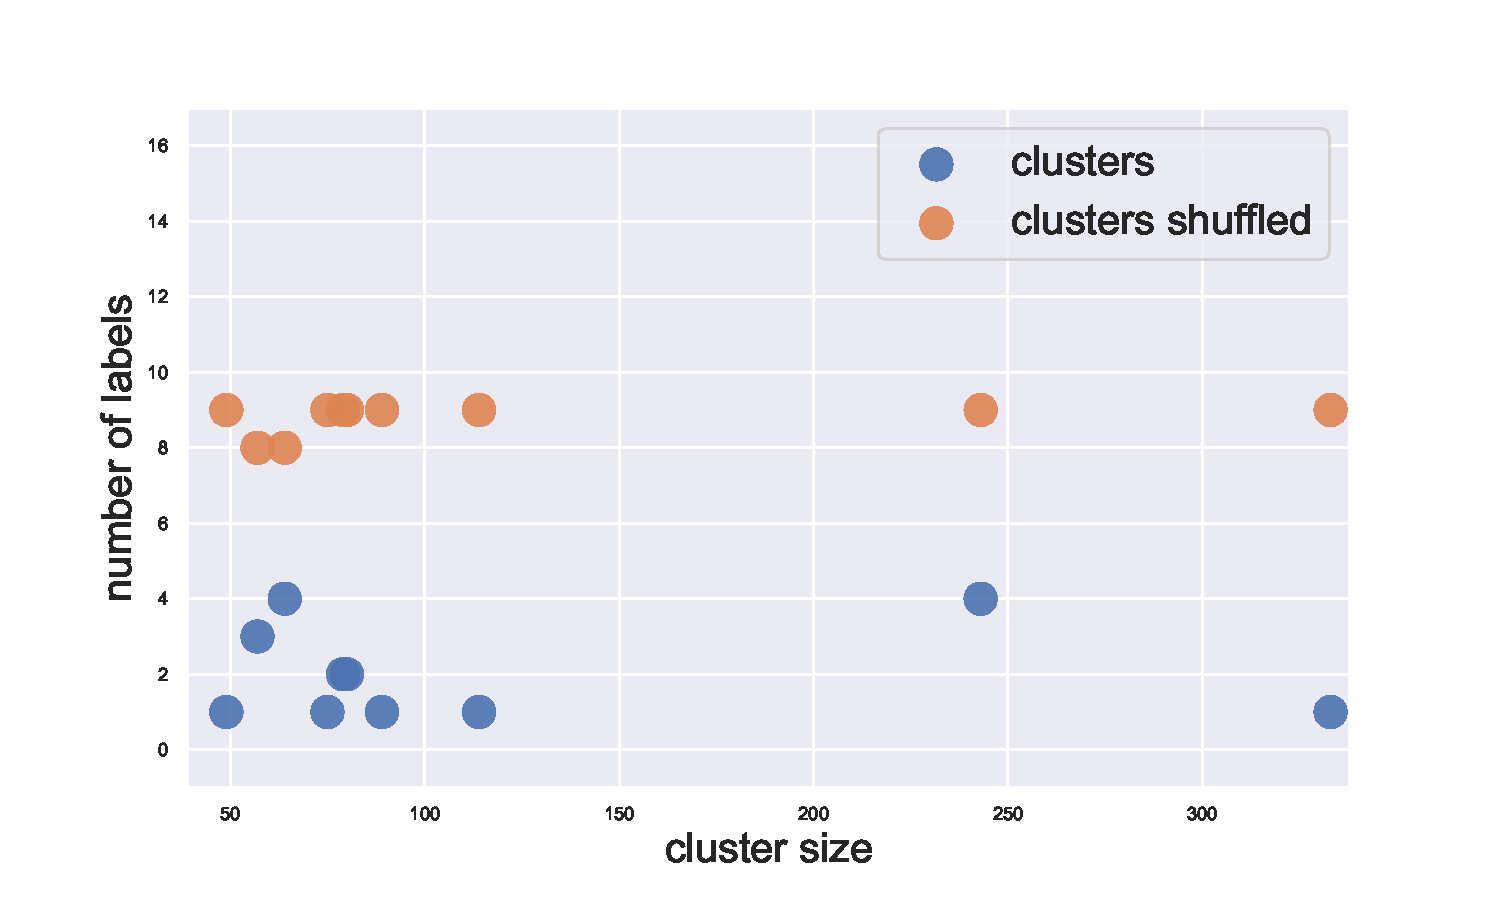
\includegraphics[width=0.9\linewidth]{pictures/topic/gtex/oversigma_10tissue/shuffledcluster_shuffle_label_size_l3_primary_site.pdf}
    \caption{Caption}
    \label{fig:topic/gtex/oversigma_10tissue/shuffledcluster_shuffle_label_size_l3_primary_site}
\end{figure}


\begin{figure}[htb!]
    \centering
    \begin{minipage}{0.45\textwidth}
    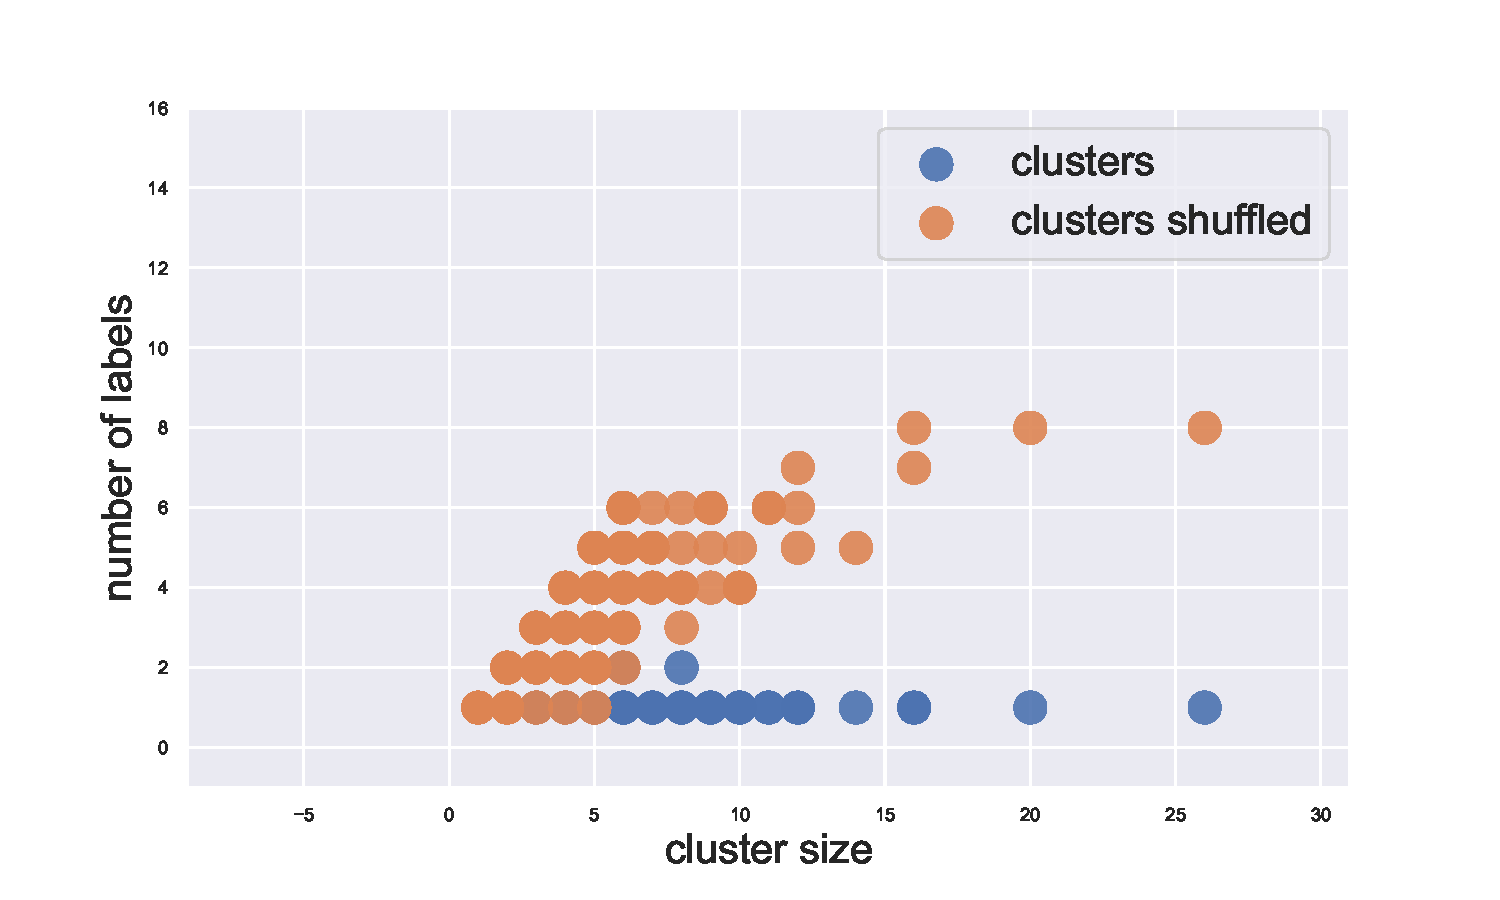
\includegraphics[width=0.9\linewidth]{pictures/topic/gtex/oversigma_10tissue/shuffledcluster_shuffle_label_size_l1_primary_site.pdf}
    \end{minipage}
    \hspace{3mm}
    \begin{minipage}{0.45\textwidth}
    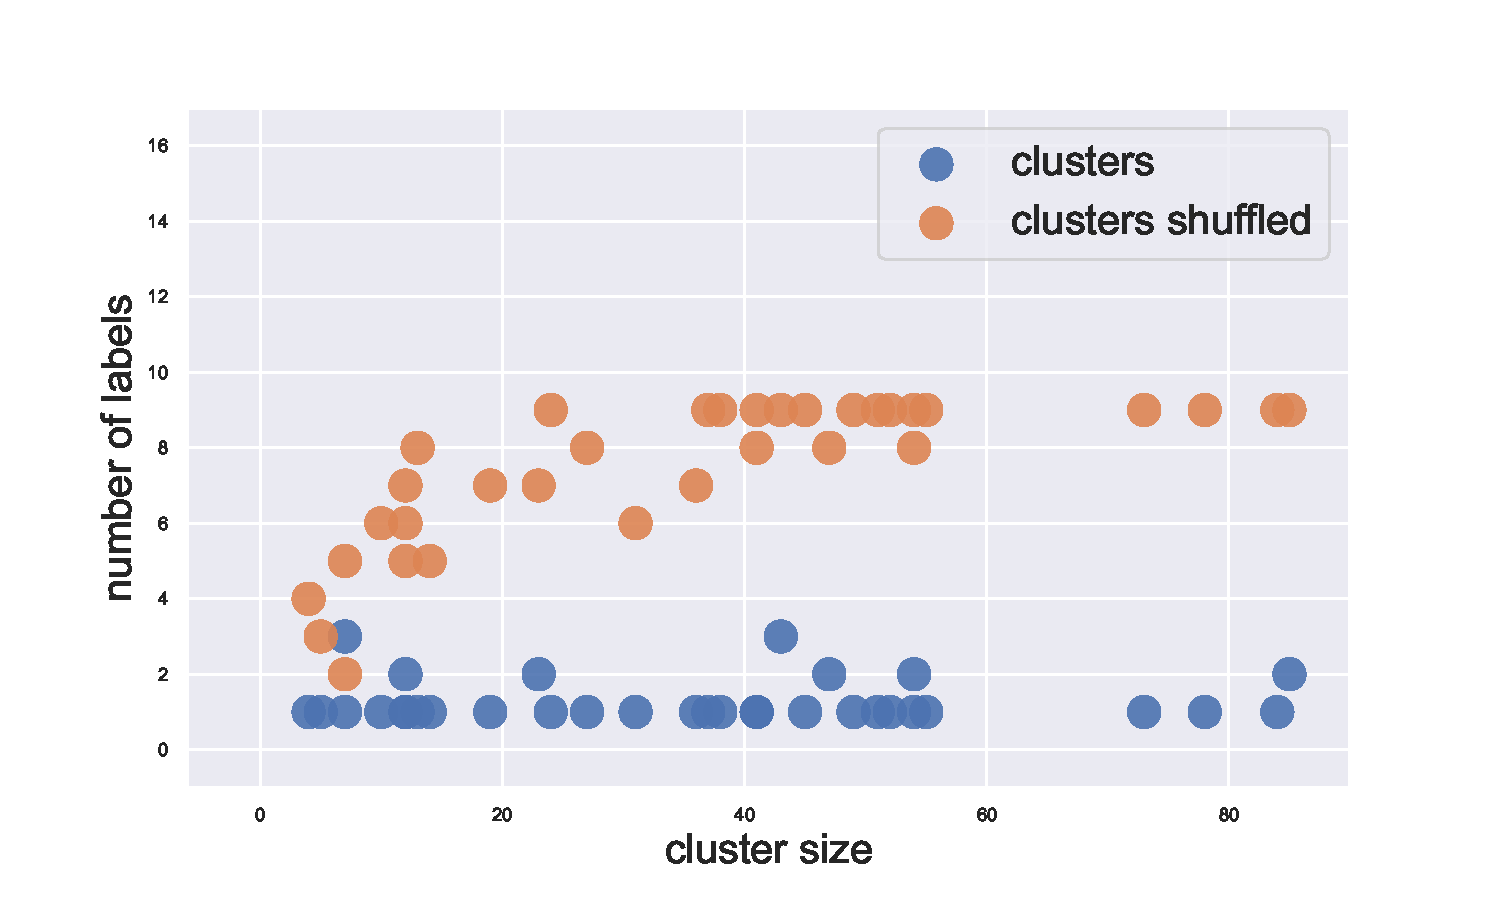
\includegraphics[width=0.9\linewidth]{pictures/topic/gtex/oversigma_10tissue/shuffledcluster_shuffle_label_size_l2_primary_site.pdf}
    \end{minipage}
    \\
    \begin{minipage}{0.45\textwidth}
    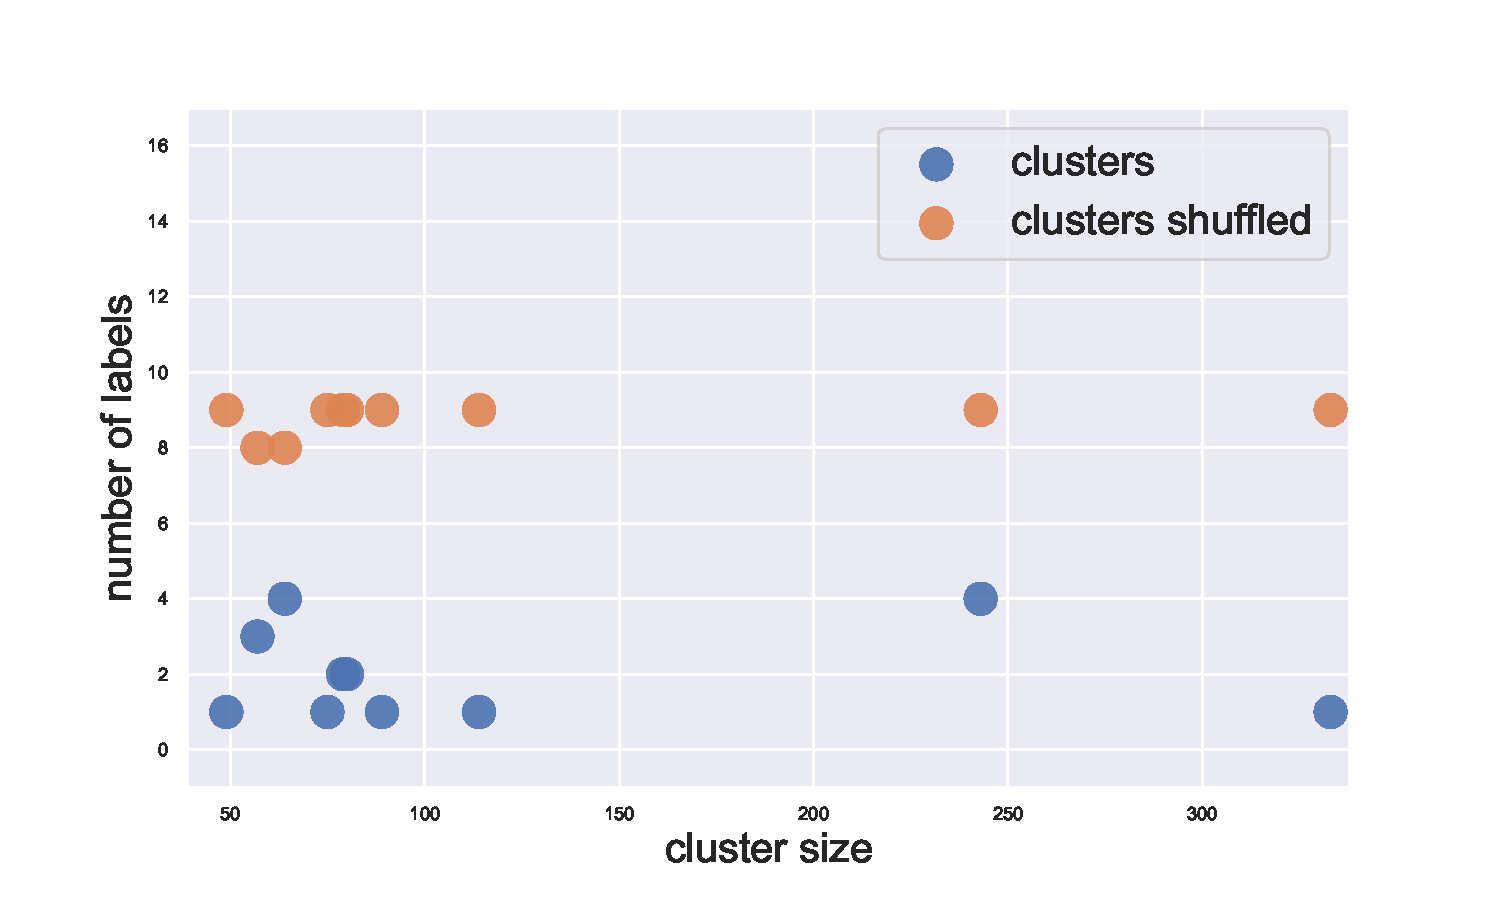
\includegraphics[width=0.9\linewidth]{pictures/topic/gtex/oversigma_10tissue/shuffledcluster_shuffle_label_size_l3_primary_site.pdf}
    \end{minipage}
    \hspace{3mm}
    \begin{minipage}{0.45\textwidth}
    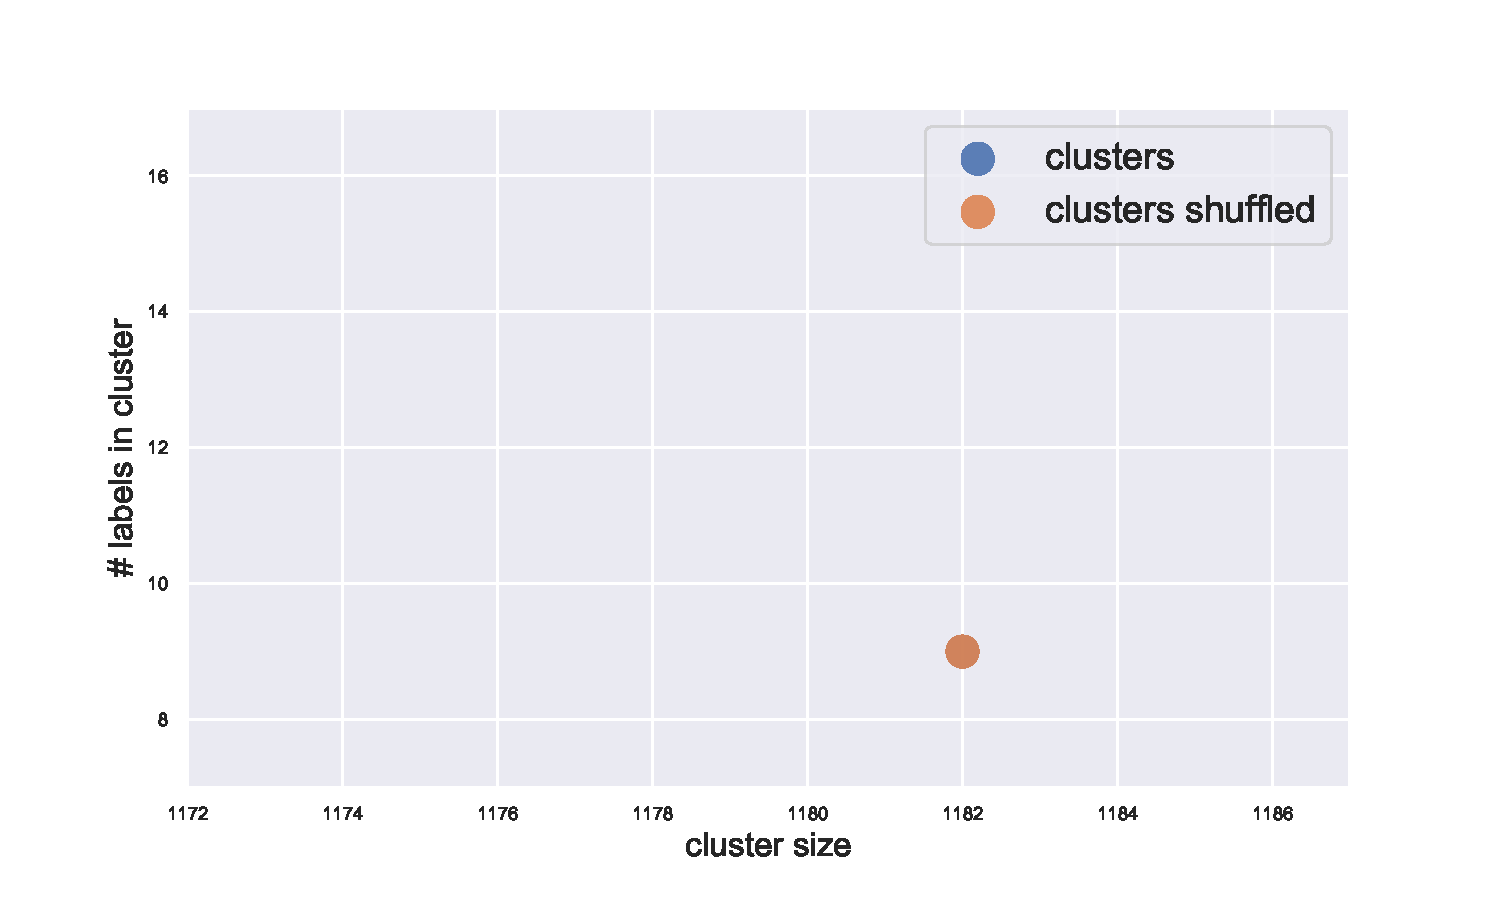
\includegraphics[width=0.9\linewidth]{pictures/topic/gtex/oversigma_10tissue/shuffledcluster_shuffle_label_size_l4_primary_site.pdf}
    \end{minipage}
\end{figure}

\begin{figure}[htb!]
    \centering
    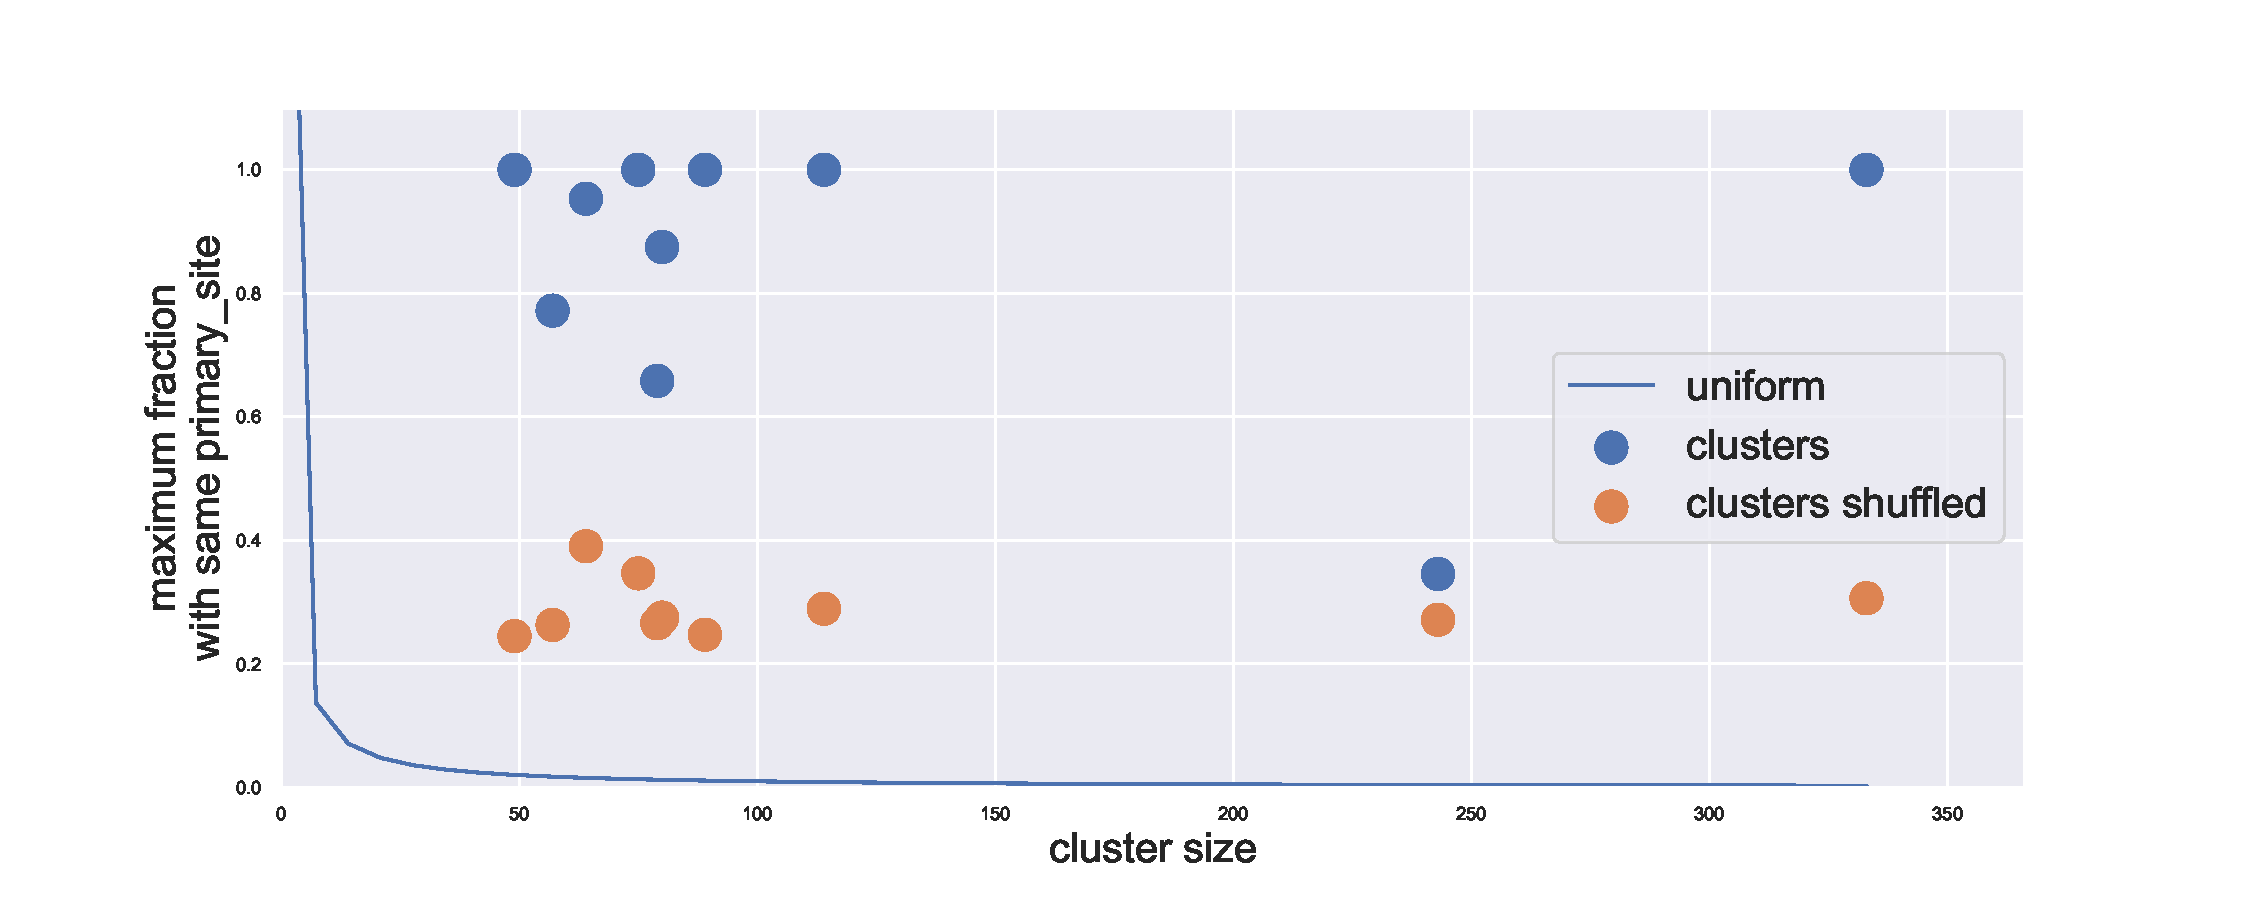
\includegraphics[width=0.9\linewidth]{pictures/topic/gtex/oversigma_10tissue/shuffledclusterhomosize_l3_primary_site.pdf}
    \caption{Caption}
    \label{fig:topic/gtex/oversigma_10tissue/shuffledclusterhomosize_l3_primary_site}
\end{figure}


\begin{figure}[htb!]
    \centering
    \begin{minipage}{0.45\textwidth}
    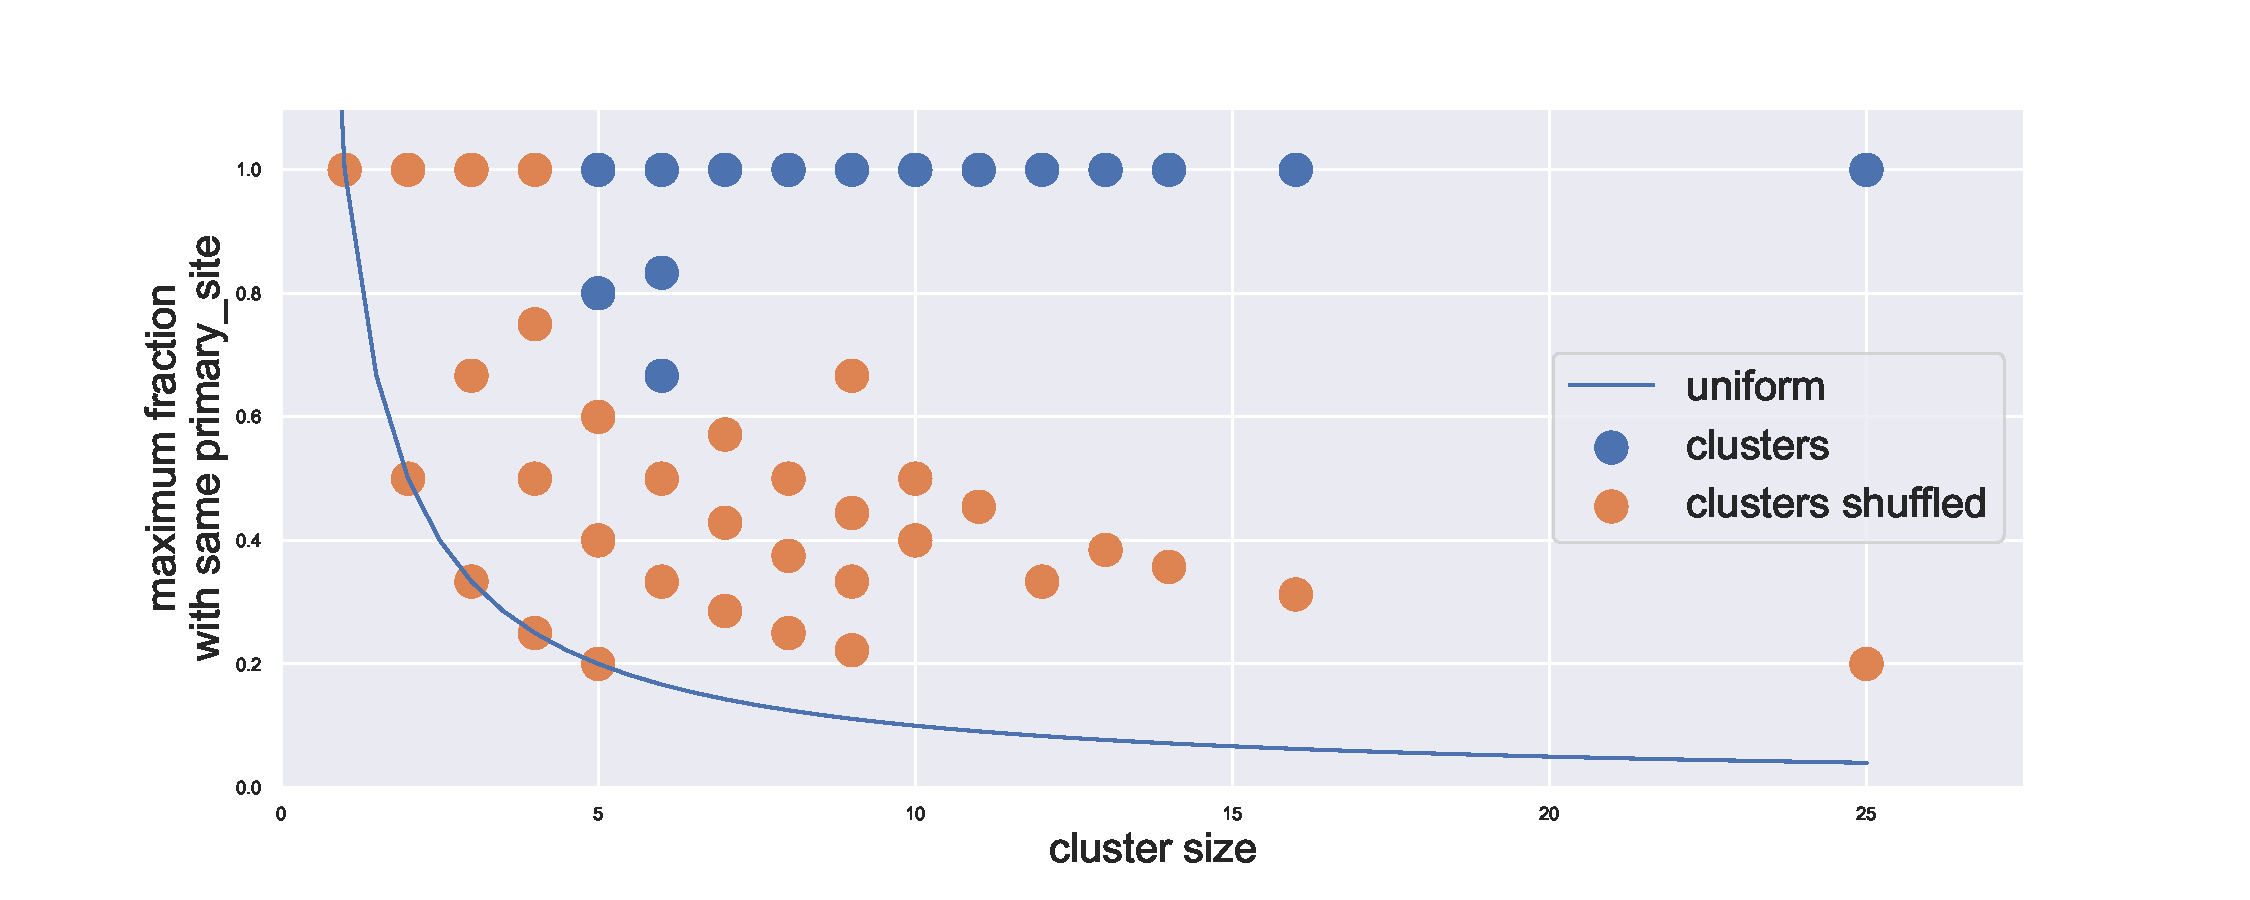
\includegraphics[width=0.9\linewidth]{pictures/topic/gtex/oversigma_10tissue/shuffledclusterhomosize_l1_primary_site.pdf}
    \end{minipage}
    \hspace{3mm}
    \begin{minipage}{0.45\textwidth}
    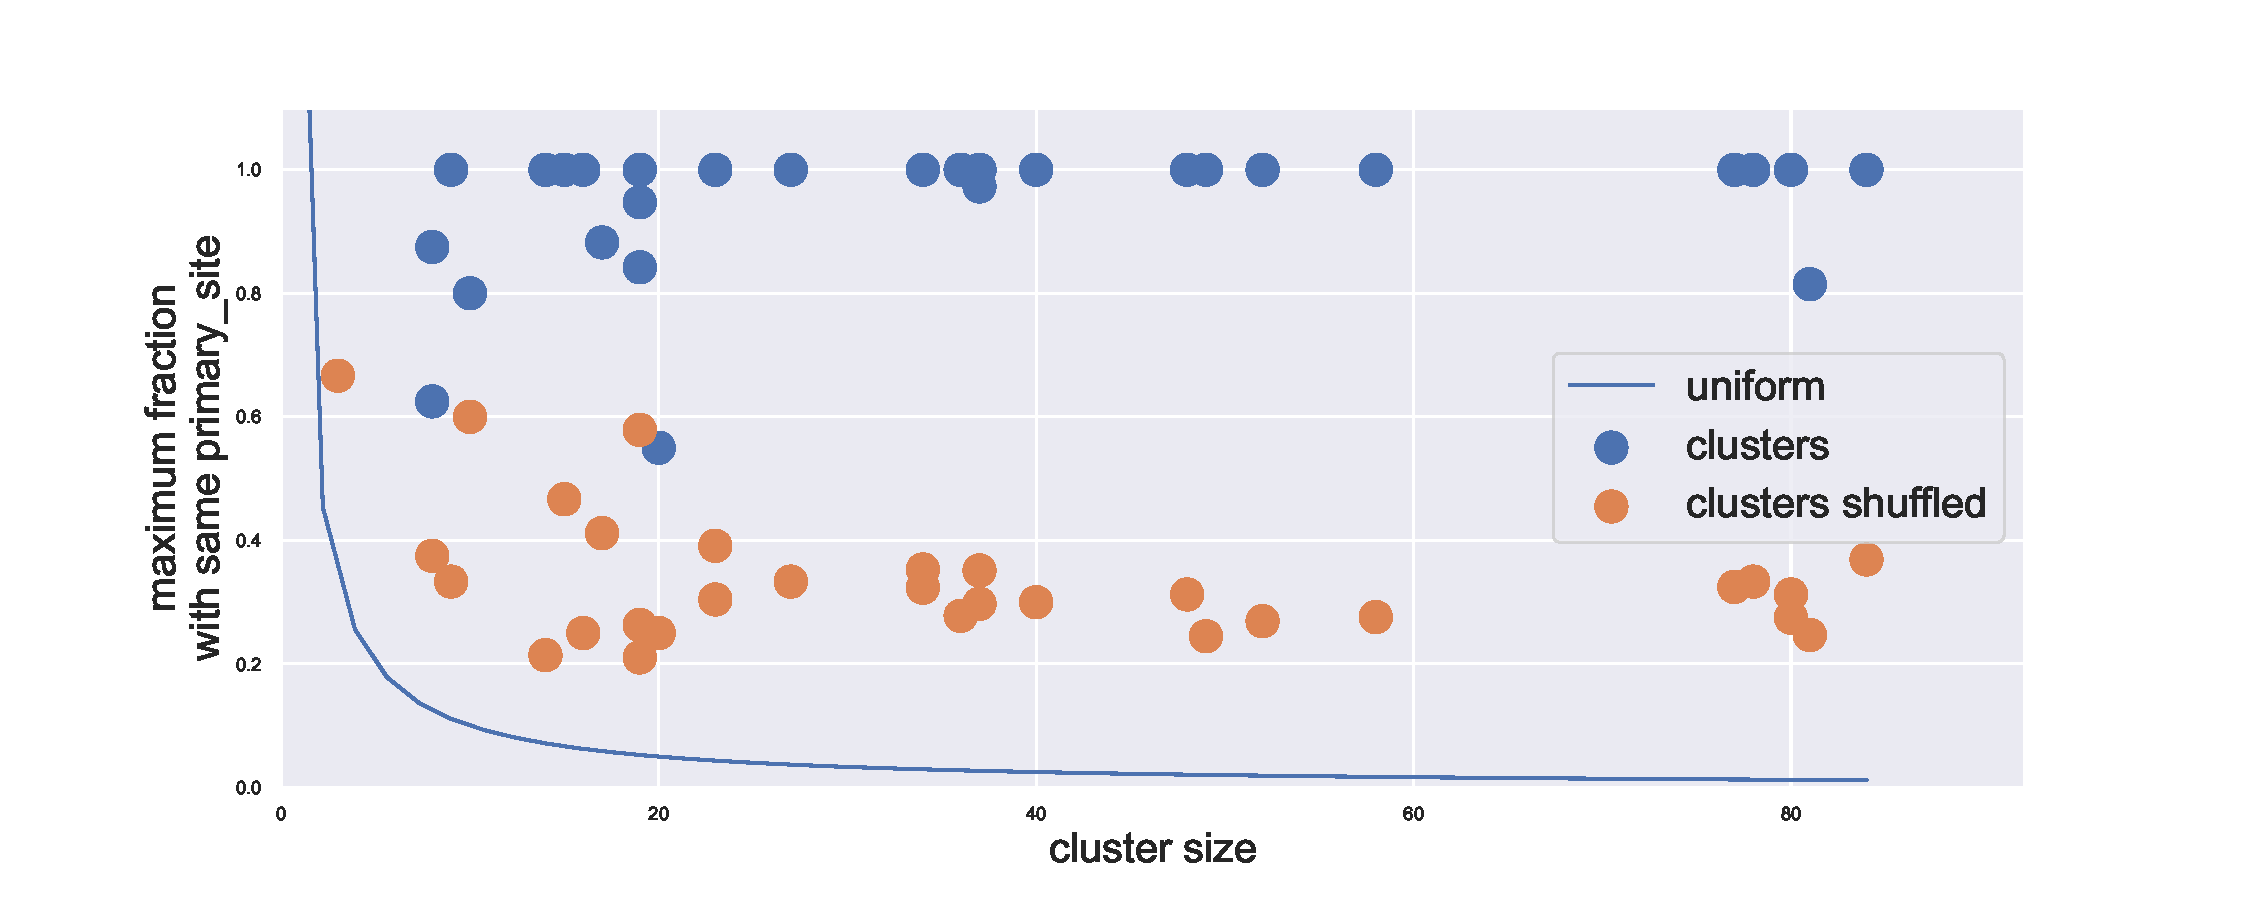
\includegraphics[width=0.9\linewidth]{pictures/topic/gtex/oversigma_10tissue/shuffledclusterhomosize_l2_primary_site.pdf}
    \end{minipage}
    \\
    \begin{minipage}{0.45\textwidth}
    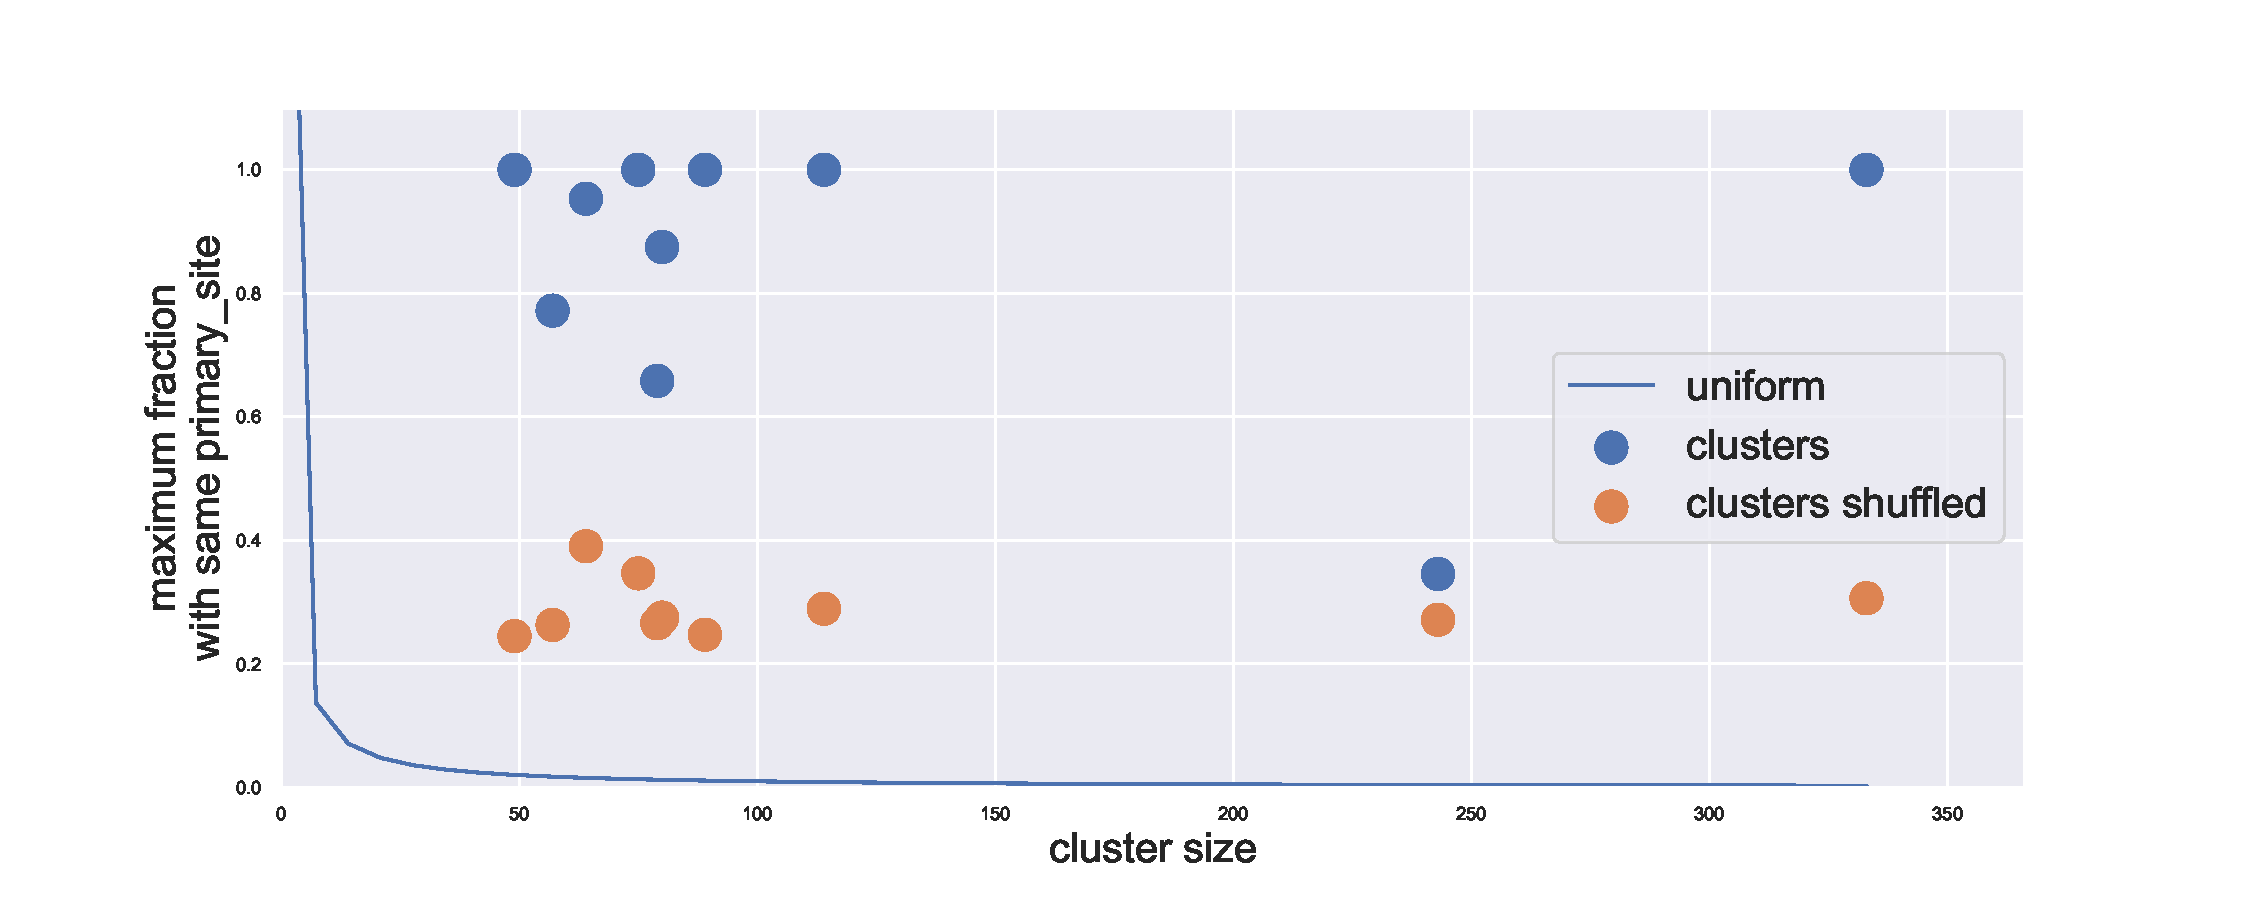
\includegraphics[width=0.9\linewidth]{pictures/topic/gtex/oversigma_10tissue/shuffledclusterhomosize_l3_primary_site.pdf}
    \end{minipage}
    \hspace{3mm}
    \begin{minipage}{0.45\textwidth}
    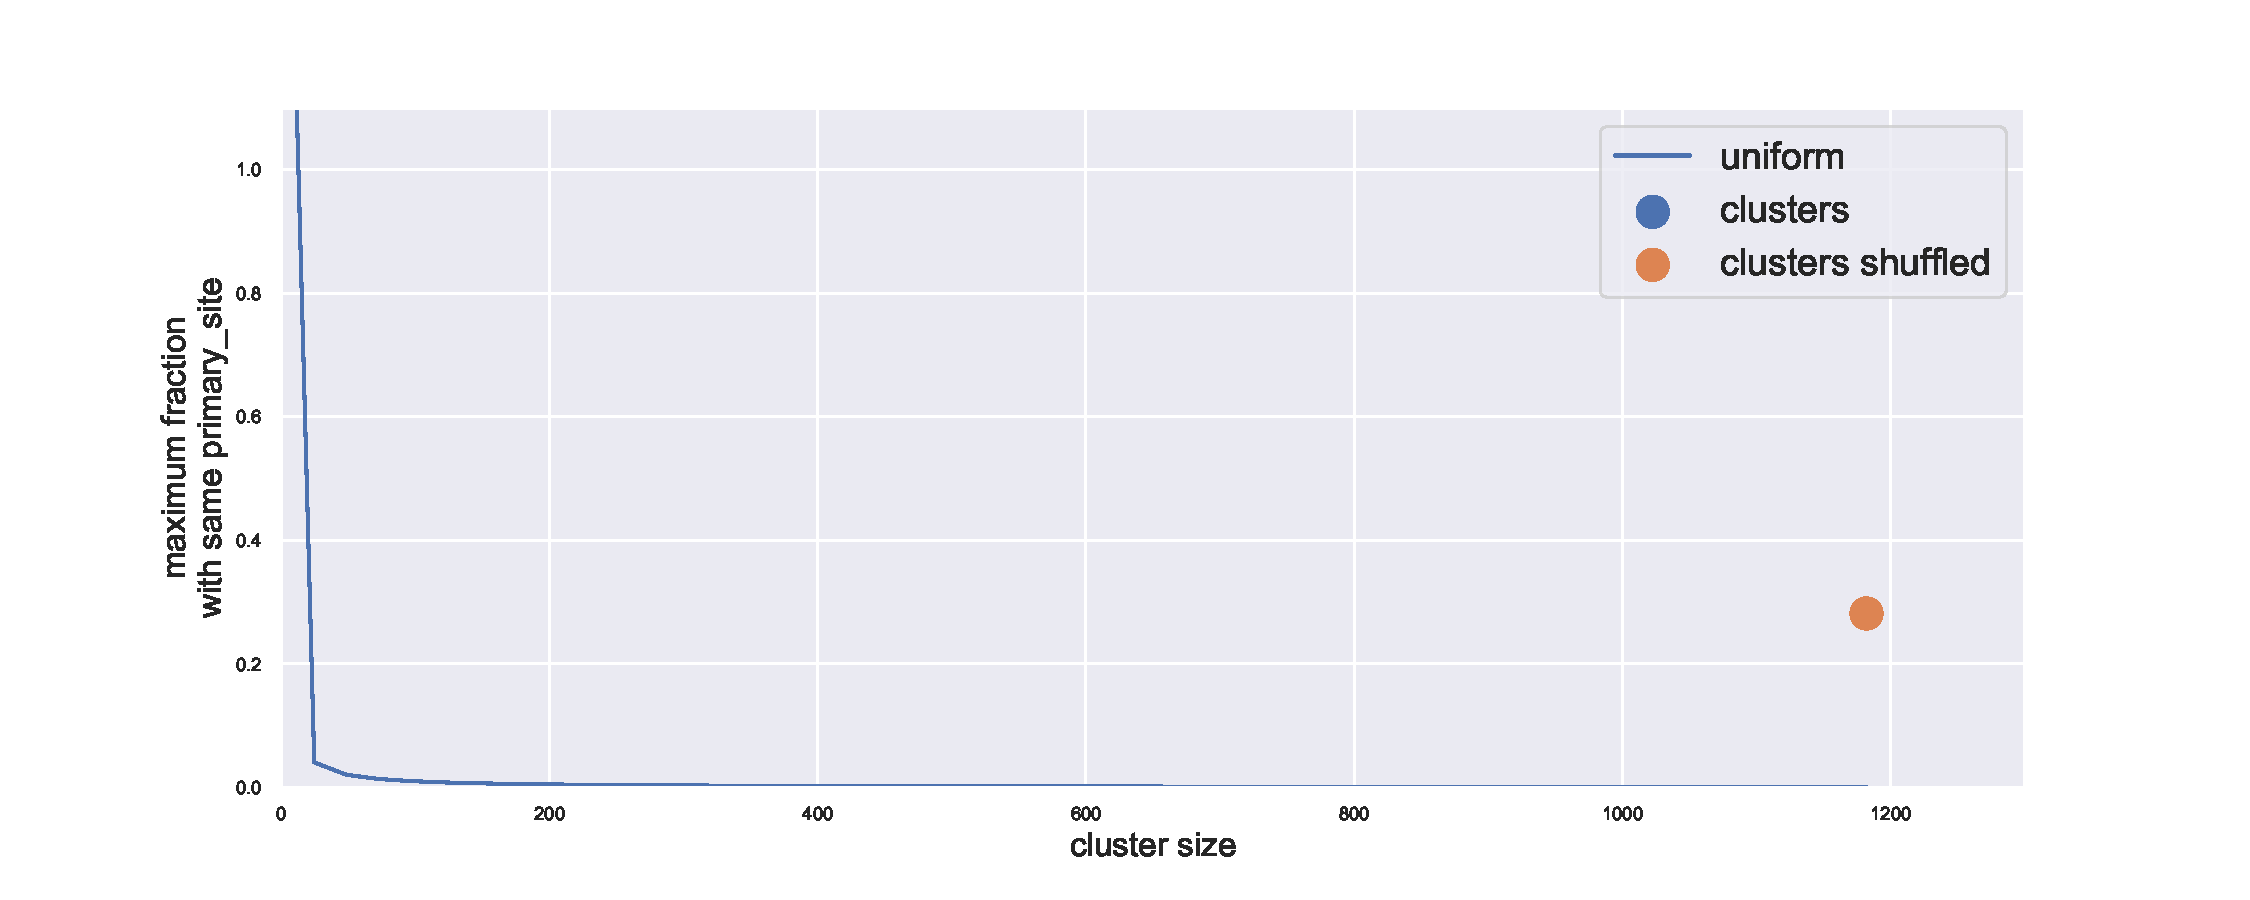
\includegraphics[width=0.9\linewidth]{pictures/topic/gtex/oversigma_10tissue/shuffledclusterhomosize_l4_primary_site.pdf}
    \end{minipage}
\end{figure}


\subsection{Shuffling}

\begin{figure}[htb!]
    \centering
    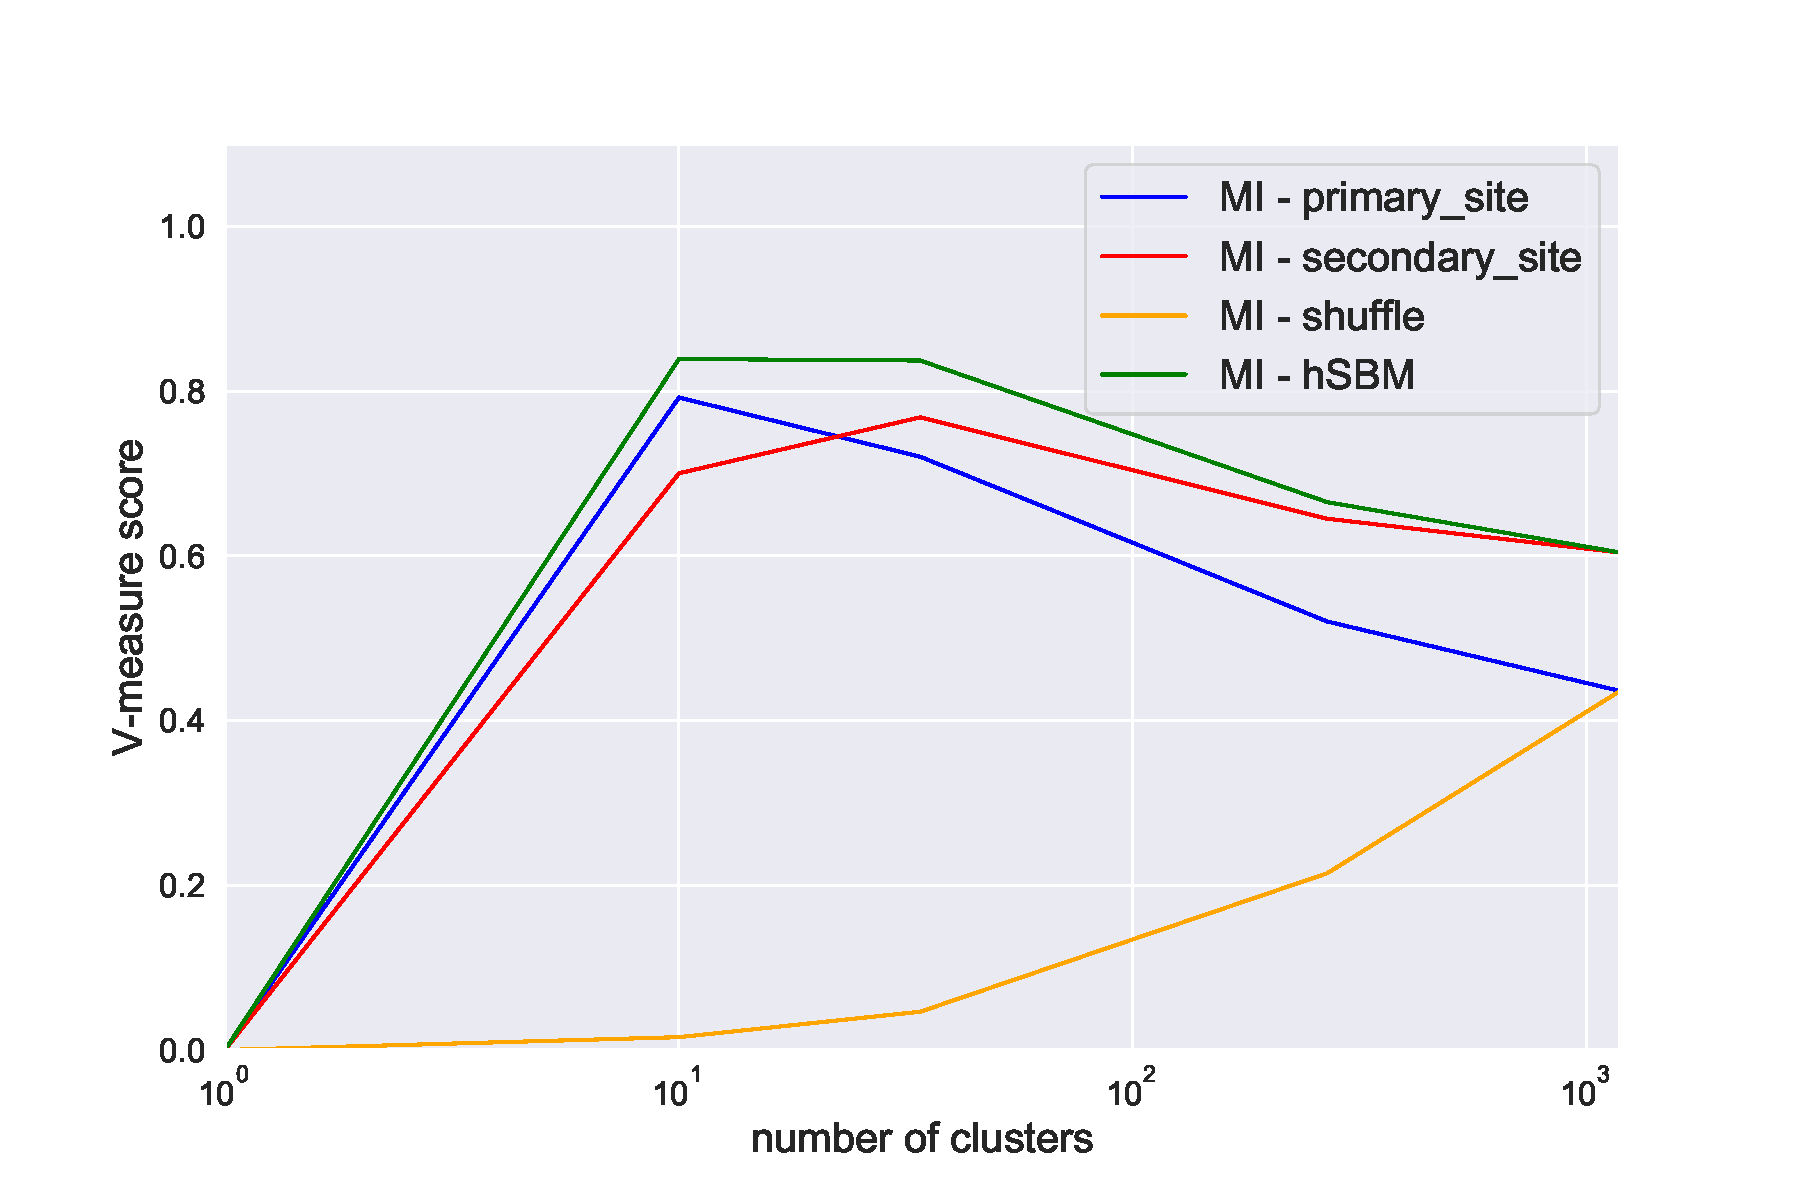
\includegraphics[width=0.9\linewidth]{pictures/topic/gtex/oversigma_10tissue/metric_scores_shuffle.pdf}
    \caption{Scores across hierarchy. The scored is compared with some random labels}
    \label{fig:topic/gtex/oversigma_10tissue/metric_scores_shuffle}
\end{figure}

\subsection{Standard algorithms}

\begin{figure}[htb!]
    \centering
    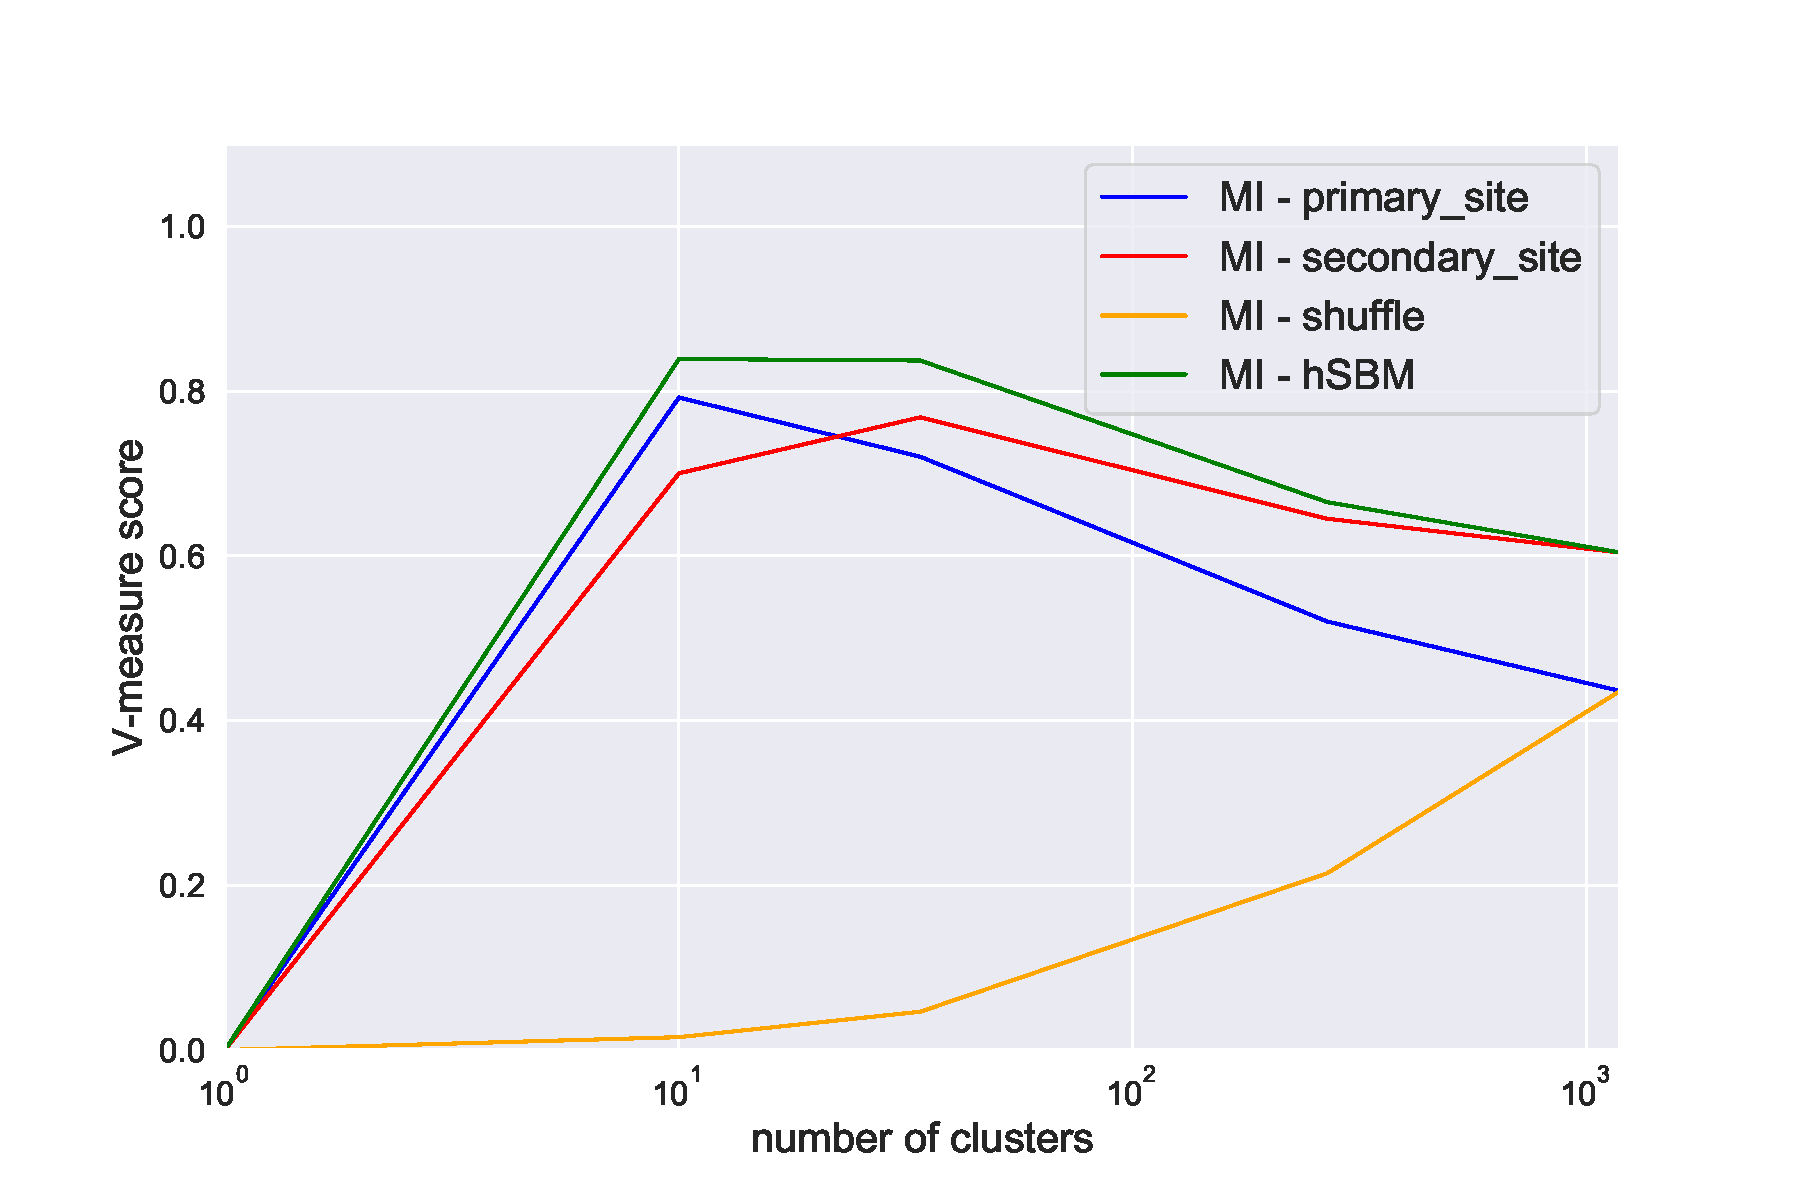
\includegraphics[width=0.9\linewidth]{pictures/topic/gtex/oversigma_10tissue/metric_scores_shuffle.pdf}
    \caption{Scores across hierarchy. The scored is compared with some random labels}
    \label{fig:topic/gtex/oversigma_10tissue/metric_scores_shuffle}
\end{figure}

\begin{figure}[htb!]
    \centering
    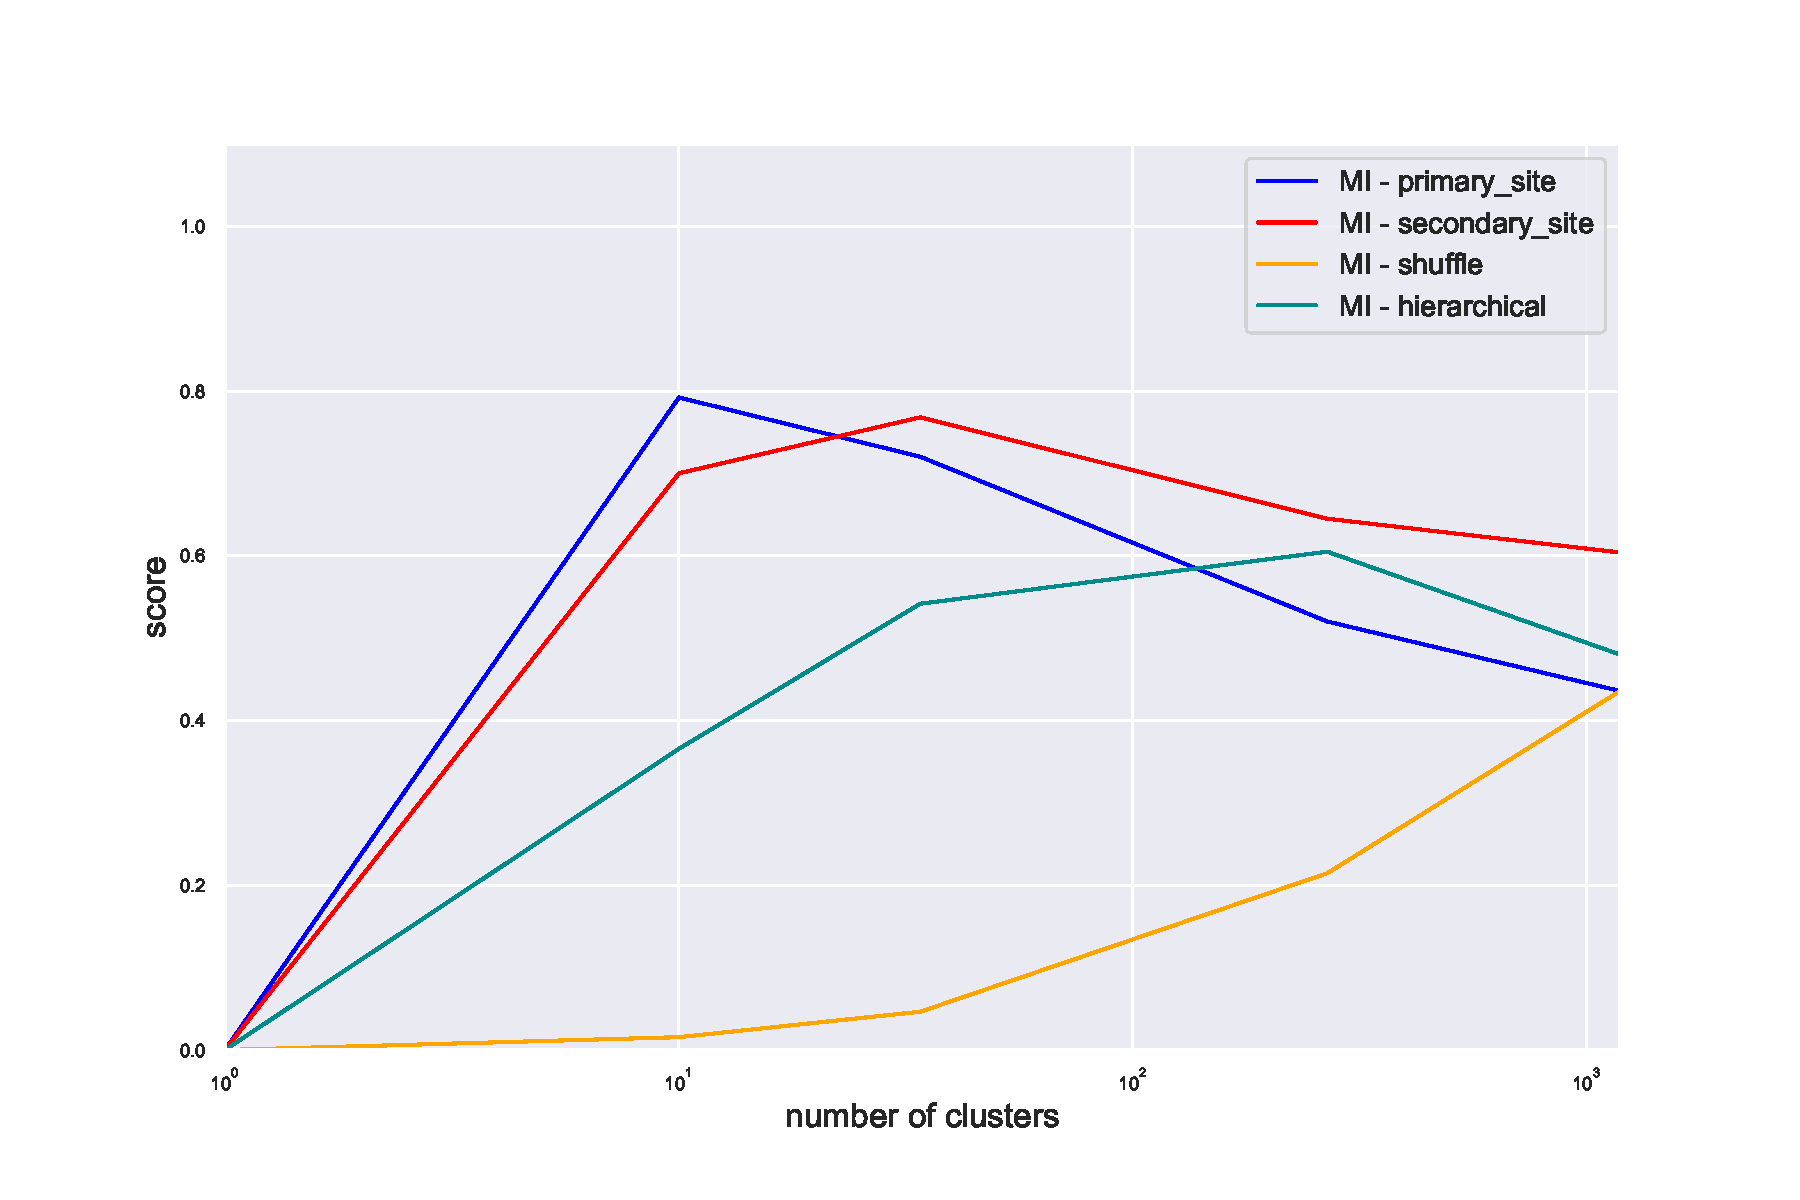
\includegraphics[width=0.9\linewidth]{pictures/topic/gtex/oversigma_10tissue/metric_scores_hier.pdf}
    \caption{Scores across hierarchy. The scored is compared with some random labels}
    \label{fig:topic/gtex/oversigma_10tissue/metric_scores_hier}
\end{figure}

\begin{figure}[htb!]
    \centering
    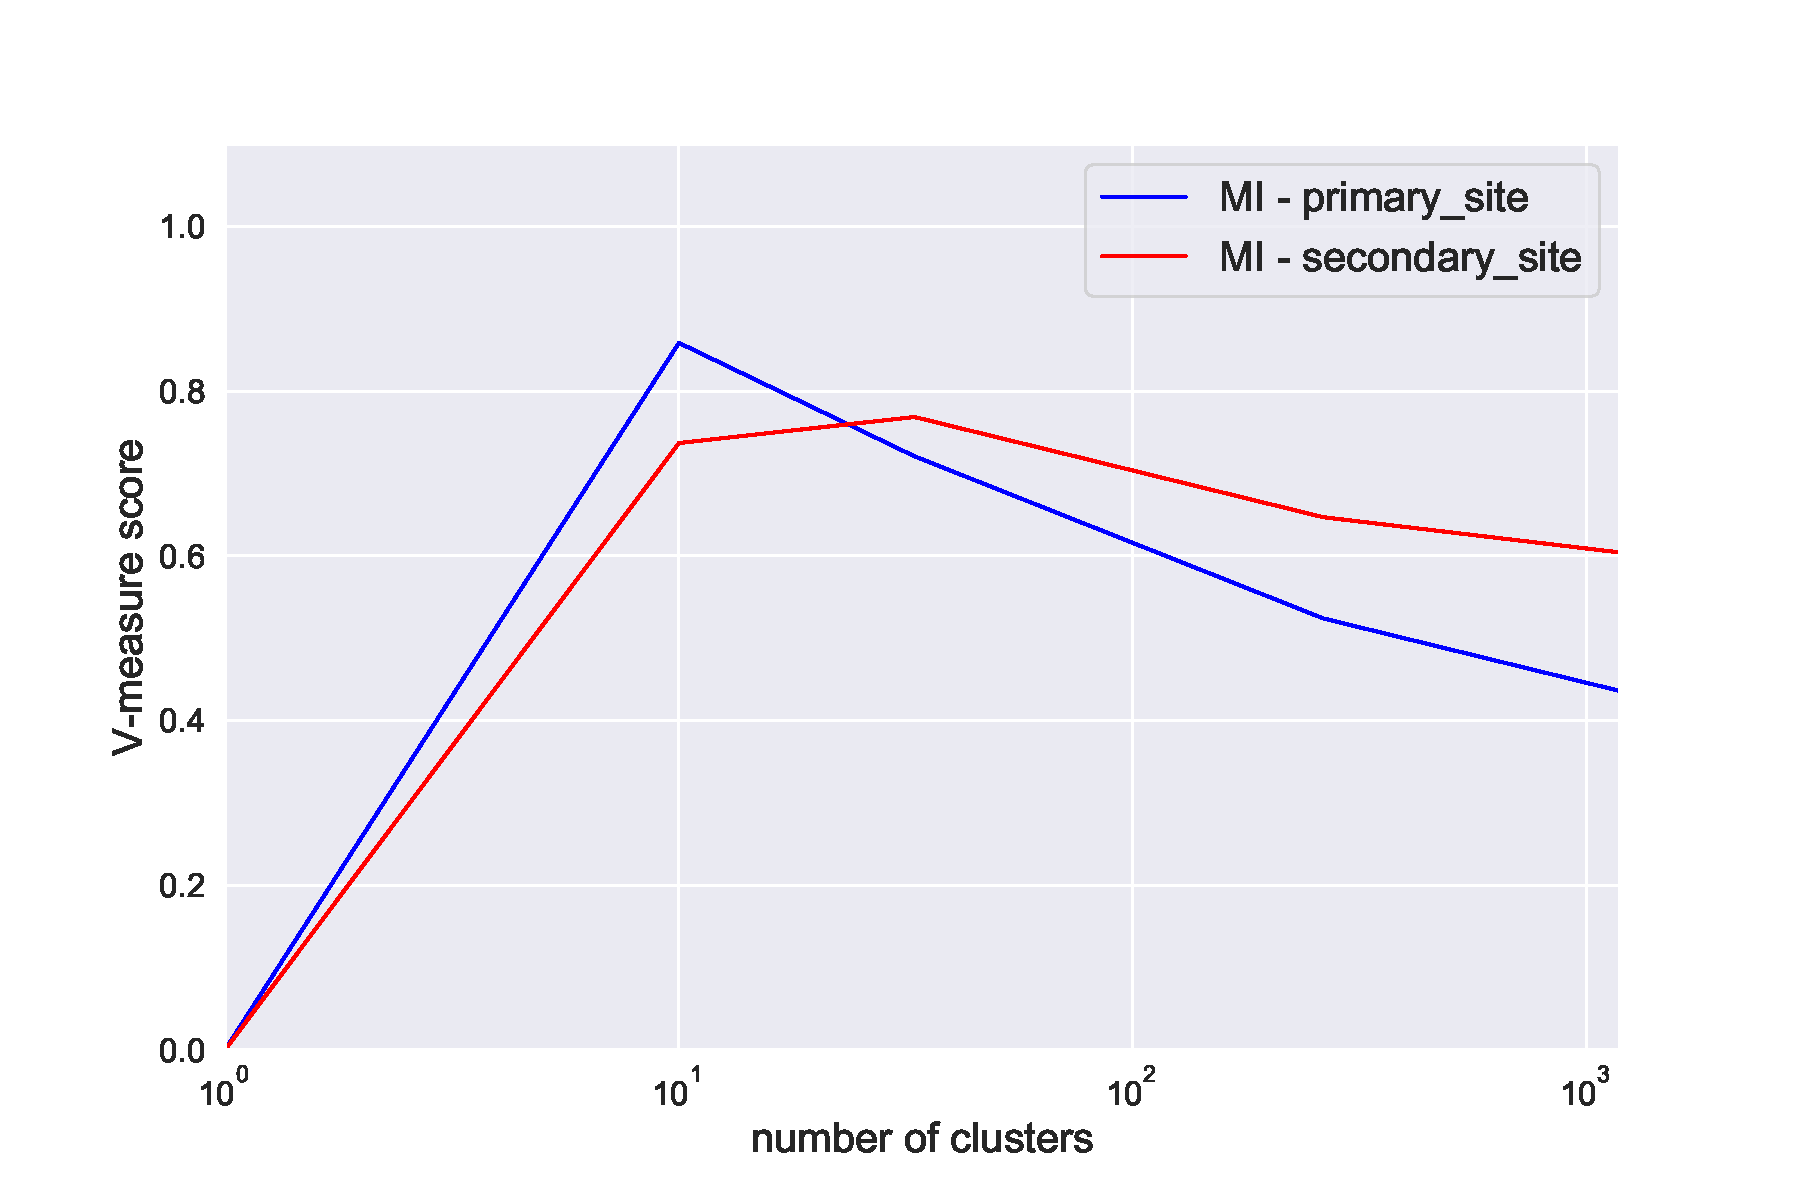
\includegraphics[width=0.9\linewidth]{pictures/topic/gtex/oversigma_10tissue/metric_scores.pdf}
    \caption{Scores across hierarchy. The scored is compared with some random labels}
    \label{fig:topic/gtex/oversigma_10tissue/metric_scores}
\end{figure}